\chapter{图的表示与计算}
\label{chap:graph-theory}

把四个变量之间的局部约束画成一张图以后，能否从一个变量走到另一个变量？
哪些变量可以分开处理，哪些选择能获得最优性证书？若在每个顶点放一个数，
邻域汇总又会保留或抹去什么？这些问题共享连接结构，却需要不同的计算规则。
本章把图本身作为研究对象，利用已有的集合、逻辑与线性代数工具，建立路径查询、
结构分解、离散选择及图上函数的运算。后续第~\ref{chap:causal-inference}章再说明
图怎样表达生成机制，以及什么条件下图分离能够推出概率独立。本章的图判据与局部
计算先独立成立；局部传播是否精确，还须检查函数分解与运算规则。

继续使用第~\ref{chap:combinatorics}章的四个二值变量
\[
  z_i\in\{0,1\},\qquad i\in V=\{1,2,3,4\}.
\]
式~\eqref{eq:comb-running-cnf}的前两个子句共同涉及\(z_1,z_2\)，
第三个子句涉及\(z_1,z_3\)，三变量子句
\(\neg z_4\lor z_2\lor z_3\)则同时涉及\(z_2,z_3,z_4\)。
把共同出现的每一对变量连接，得到
\begin{equation}
  E=\bigl\{\{1,2\},\{1,3\},\{2,3\},\{2,4\},\{3,4\}\bigr\}.
  \label{eq:graph-theory-running-edges}
\end{equation}
图~\ref{fig:graph-theory-running-graph}中，左右两个三角形共享顶点\(2,3\)。
固定这两个变量以后，左右两侧的局部计算可以分别进行；但三元子句仍须保留，
三条两两连接并没有把它变成三个等价的二元约束。

\begin{figure}[htbp]
  \centering
  \begin{tikzpicture}[text=FigureInk,
    vertex/.style={circle,draw=FigureStroke,fill=FigureYellowFill,line width=1pt,
      minimum size=8mm,inner sep=0pt,font=\figurefont\footnotesize},
    edge/.style={draw=FigureStroke,line width=1.1pt}
  ]
    \node[vertex] (x2) at (0,1.15) {\(z_2\)};
    \node[vertex] (x3) at (0,-1.15) {\(z_3\)};
    \node[vertex] (x1) at (-2.1,0) {\(z_1\)};
    \node[vertex] (x4) at (2.1,0) {\(z_4\)};
    \draw[edge] (x1)--(x2);
    \draw[edge] (x1)--(x3);
    \draw[edge] (x2)--(x3);
    \draw[edge] (x2)--(x4);
    \draw[edge] (x3)--(x4);
  \end{tikzpicture}
  \caption{由四变量约束的作用域导出的关系图。边表示两个变量共同出现在至少一个
  约束中；共享顶点集合\(\{2,3\}\)连接左右两侧。图没有记录约束的具体真值表，
  也没有预先指定边长、容量或相似度。}
  \label{fig:graph-theory-running-graph}
\end{figure}

本章先确定图记录的对象，再沿路径检索关系。由路径得到的分隔接口，可以组织局部块；
结构抽取和消元则说明改写图时保留什么、增加什么。给定结构以后，路径、流量、树、
匹配和标签的最优选择各有自己的目标与条件。图上函数的变换还要区分两种定义域：
给每个顶点一个数，与给全部变量的一次完整赋值一个数，所需运算并不相同。
这种区分连接图谱滤波与局部精确查询，也说明前章规则信号中的变换与卷积
推广到一般连接结构时，需要重新选择哪些对象与运算。

\section{图的对象与表示}
\label{sec:graph-theory-objects-representations}

画一条线之前，需要说明它记录的是对称关系、有方向的作用，还是某个多变量函数的
作用域。确定对象以后，邻接表与矩阵只是同一结构的不同存储方式；改变顶点编号
也不应改变结构本身。这里固定这些约定，路径、优化和传播再分别使用它们。

\subsection{局部关系的对象与作用域}
\label{sec:graph-theory-local-relations}

\subsubsection{二元关系的图表示}
\label{sec:graph-theory-binary-relations}

若只需记录哪些对象直接相关，可以让每个对象对应一个顶点，让一对对象的关系对应
一条边。\term{无向图}（undirected graph）是
\(\mathcal G=(V,E)\)，其中\(V\)是有限顶点集合，\(E\)是不同顶点的无序对集合。
本章默认没有自环，也没有同一对顶点之间的平行边；允许这些情形时，要另外保存
边的身份及重数，不能继续把边集理解成普通无序对集合。

若\(\{i,j\}\in E\)，称\(i,j\)相邻，二者互为邻居。
顶点\(i\)的\term{邻域}（neighborhood）是它的全部邻居，
\term{度}（degree）是邻居的数量：
\[
  N(i)=\{j\in V:\{i,j\}\in E\},\qquad d_i=|N(i)|.
\]
贯穿图中\(N(2)=\{1,3,4\}\)、\(d_2=3\)，而
\(N(1)=\{2,3\}\)、\(d_1=2\)。度只统计直接连接，不统计经过其他顶点能够到达的对象。

关系具有方向时，使用\term{有向图}（directed graph）
\(\mathcal G=(V,A)\)，其中\(A\subseteq V\times V\)是有序对的集合，
并仍排除\((i,i)\)。弧\((i,j)\)写作\(i\to j\)，不自动包含反向弧。
入邻域\(N^-(j)=\{i:i\to j\}\)与出邻域\(N^+(j)=\{i:j\to i\}\)
分别记录指向本点和从本点指出的对象；它们的大小称为
\term{入度}（in-degree）和\term{出度}（out-degree）。
有向图中也常把入邻居称为父节点，把出邻居称为子节点。这些名称只说明连接方向；
一般有向边可以表示计算依赖或允许通行的方向，不能只凭箭头赋予因果意义。

在结构边上还可以指定\term{权重}（weight），即每条边附带的数值。
无向权重满足\(w_{i,j}=w_{j,i}\)，有向权重允许方向不同。
有向与无向描述方向，加权与无权描述是否附带数值，是能够组合的两个属性。
边长越大表示经过它的成本越高，容量越大表示允许通过的总量越多，
相似度越大则通常表示两端越接近；同一个数字不能未经转换同时充当这三种量。

结构存在也不等于权重非零。本章允许零权结构边，另把无向非负权图中的
\[
  E_+=\{\{i,j\}\in E:w_{i,j}>0\}
\]
称为\term{正权支撑}（positive-weight support）。
例如两顶点之间存在一条权重为零的边，结构上仍相邻，但在线性加权汇总中互不贡献。
因此后面的谱与扩散结论使用支撑图\(\mathcal G_+=(V,E_+)\)，
而结构路径查询是否使用零权边，要由查询规则另行决定。

只研究部分对象时，不能无声改掉它们之间的关系。给定\(U\subseteq V\)，
保留\(U\)及原图中两端都属于\(U\)的全部边或弧，所得图称为
\term{诱导子图}（induced subgraph），记作\(\mathcal G[U]\)。
贯穿图在\(\{1,2,3\}\)上的诱导子图必须保留三条边；只留下\(1-2-3\)
是一个子图，却不是该顶点集上的诱导子图。

\subsubsection{高阶关系的因子表示}
\label{sec:graph-theory-higher-order-scopes}

三元子句\(\neg z_4\lor z_2\lor z_3\)要求同时查看三个变量。
这种局部函数称为因子（factor），它依赖的变量集合称为作用域（scope）。
要保留“共同属于同一个因子”的信息，可以使用\term{超图}（hypergraph）：
每条超边是一个顶点子集，不限于两个顶点；超边\(\{2,3,4\}\)在这里记录三元作用域。
函数值仍须另外保存，超边本身也不是约束真值表。

另一种表示把变量和因子分成两组，只在变量属于因子作用域时连边。
两组顶点内部都没有边的图称为\term{二部图}（bipartite graph）；
这样得到的因子图（factor graph）用方形顶点保存因子的身份，用圆形顶点保存变量。
若只保留变量，并把每个因子作用域内的变量两两相连，得到
\term{原始关系图}（primal graph），也简称原始图。
贯穿图正是按这条规则由原子句得到的。

图~\ref{fig:graph-theory-factor-scope}比较两种表示。一个三元因子和三个二元因子
可以产生同一个三角形原始图，但它们的函数族一般不同。
例如二值三元约束“恰有偶数个变量等于\(1\)”允许
\(000,011,101,110\)。每一对变量的四种取值都在某个允许配置中出现；
若只保留这三个二元允许关系，它们便不再排除任何配置，错误地允许了\(001\)。
两两关系无法恢复被丢失的三元相容条件。

\begin{figure}[htbp]
  \centering
  \begingroup
% Local styles; callers keep this input inside a group.
\tikzset{
  reader vertex/.style={circle,draw=FigureStroke,fill=white,line width=1pt,
    minimum size=7mm,inner sep=0pt,font=\figurefont\footnotesize,text=FigureInk},
  reader factor/.style={rectangle,draw=FigureStroke,fill=FigureYellowFill,
    line width=1pt,minimum size=8mm,inner sep=2pt,font=\figurefont\footnotesize},
  reader edge/.style={draw=FigureStroke,line width=1.1pt},
  reader arrow/.style={reader edge,-{Stealth[length=2.2mm,width=1.4mm]}},
  reader label/.style={font=\figurefont\footnotesize,text=FigureInk},
  reader note/.style={reader label,fill=white,inner sep=1pt},
  reader highlight/.style={draw=FigureYellow,line width=1.1pt},
  reader auxiliary/.style={draw=FigureMuted,line width=0.6pt,dashed}
}

\begin{tikzpicture}[text=FigureInk]
  \node[reader label] at (0,1.35) {(a) 三元因子};
  \node[reader factor] (f) at (0,0) {\(\phi_{2,3,4}\)};
  \node[reader vertex] (a) at (-1.35,0) {\(z_2\)};
  \node[reader vertex] (b) at (0,-1.05) {\(z_3\)};
  \node[reader vertex] (c) at (1.35,0) {\(z_4\)};
  \draw[reader edge] (a)--(f)--(c);
  \draw[reader edge] (b)--(f);
  \node[reader label] at (4.8,1.35) {(b) 原始关系图};
  \node[reader vertex] (x) at (3.45,0) {\(z_2\)};
  \node[reader vertex] (y) at (4.8,-1.05) {\(z_3\)};
  \node[reader vertex] (z) at (6.15,0) {\(z_4\)};
  \draw[reader edge] (x)--(y)--(z)--(x);
\end{tikzpicture}
\endgroup

  \caption{三元因子与原始关系图。左侧方框是同一个依赖\(z_2,z_3,z_4\)的函数，
  连线表示作用域归属；右侧只保留变量共同出现的两两关系。右侧三条边不是把三元
  函数分解成三个二元函数的等价变换，也不能恢复原函数的数值。}
  \label{fig:graph-theory-factor-scope}
\end{figure}

\subsection{图关系的矩阵表示}
\label{sec:graph-theory-matrix-representations}

遍历要快速取出邻居，线性汇总要快速相乘，边差分还要逐边保留端点。
邻接表、邻接矩阵和关联矩阵分别直接支持这三种操作。
邻接表为每个顶点存实际邻居及其边属性，空间为\(O(|V|+|E|)\)；
无向边在两个端点各存一次只改变常数。稠密邻接矩阵则为每一对顶点预留一个位置。

固定顶点次序\(1,\ldots,n\)，\term{邻接矩阵}（adjacency matrix）
\(\bm A\in\mathbb R^{n\times n}\)的条目为
\[
  a_{i,j}=
  \begin{cases}
    w_{i,j},&\{i,j\}\in E\quad\text{或}\quad(i,j)\in A,\\
    0,&\text{其他情形}.
  \end{cases}
\]
无权边取权重\(1\)。有向情形约定行是起点、列是终点，因此
\((\bm A\bm f)_i=\sum_{j\in N^+(i)}w_{i,j}f_j\)
汇总出邻居的值；若要把每个起点的值沿出弧发送到终点，应使用
\(\bm A^\top\bm f\)。无向图中矩阵对称，两种读法才重合。
贯穿图对应
\begin{equation}
  \bm A=
  \begin{bmatrix}
    0&1&1&0\\
    1&0&1&1\\
    1&1&0&1\\
    0&1&1&0
  \end{bmatrix}.
  \label{eq:graph-theory-running-adjacency}
\end{equation}
例如\(\bm f=(1,2,3,4)^\top\)给出
\(\bm A\bm f=(5,8,7,5)^\top\)。这是顶点值的线性汇总，
不等于在全部变量配置上求和；后者还需要明确局部因子。
允许零权边时，矩阵条目\(0\)不能区分无边与零权边，必须另存边集或结构掩码
\(m_{i,j}=\mathbb I\{\text{存在相应结构边}\}\)。

要计算每条边两端的差，给每条无向边任选临时方向，构造
\term{关联矩阵}（incidence matrix）
\(\bm B\in\mathbb R^{|V|\times|E|}\)。
边\(e:i\to j\)对应列在\(i\)处取\(1\)，在\(j\)处取\(-1\)，其余为零。
于是\((\bm B^\top\bm f)_e=f_i-f_j\)。
若\(\bm W_E=\operatorname{diag}(w_e:e\in E)\)，
\(\bm B\bm W_E\bm B^\top\)先求边差、按权缩放，再汇总回顶点。
反转某些临时方向相当于\(\bm B'=\bm B\bm R\)，其中
\(\bm R\)为对角元取\(\pm1\)的对角矩阵。
由于\(\bm R\bm W_E\bm R=\bm W_E\)，这个无向加权差分算子不随临时方向改变。
这并没有消除真正有向图中的方向，二者不能混用。

\subsection{顶点重编号下的结构同一性}
\label{sec:graph-theory-graph-isomorphism}

矩阵的位置依赖编号，图的连接关系却不应依赖编号。
两图\(\mathcal G=(V,E)\)、\(\mathcal G'=(V',E')\)若存在双射
\(\rho:V\to V'\)，使
\[
  \{i,j\}\in E
  \quad\Longleftrightarrow\quad
  \{\rho(i),\rho(j)\}\in E',
\]
就称为\term{同构}（isomorphic）：忽略顶点名称后，两图的连接完全相同。
有向图要保有序弧，加权图还要保对应权重，带属性图则须说明哪些属性也要求保持。
设置换矩阵满足\((\bm P\bm f)_{\rho(i)}=f_i\)，重编号对应
\begin{equation}
  \bm A'=\bm P\bm A\bm P^\top.
  \label{eq:graph-theory-adjacency-relabel}
\end{equation}
这是置换共轭，只挪动坐标位置，不把两个顶点的值混合。
第~\ref{chap:matrix-analysis}章的一般相似变换允许混合坐标，
所以不能把任意换基都解释成图重编号。

数值矩阵单独判同构，还要求它能恢复结构边。
无权图或所有结构边权非零时，式~\eqref{eq:graph-theory-adjacency-relabel}
给出矩阵判据；允许零权结构边时，还须验证
\(\bm M'=\bm P\bm M\bm P^\top\)。
两顶点空图与两顶点零权单边图都可有\(\bm A=\bm0\)，但前者不相邻、后者相邻。

同构必有相同邻接谱，因为置换共轭是相似变换；逆命题不成立。
例如四叶星图\(K_{1,4}\)与“四环加一个孤立顶点”都有邻接特征值
\(2,-2,0,0,0\)。前者的非零特征值来自中心与四个叶顶点的汇总，
后者的四环特征值为\(2,0,0,-2\)，再加孤立点的零值。
一图连通、另一图不连通，故不同构。这里比较的是邻接谱；
后文不同算子的谱也必须指明算子，不能只说“两个图的频率相同”。
图上顶点函数随编号怎样变化，将在第~\ref{sec:graph-theory-vertex-functions}节
用这里的置换关系检验。

\section{图上的关系、路径和遍历}
\label{sec:graph-theory-paths-traversal}

顶点不相邻，并不表示二者毫无联系：关系可以经其他顶点延伸。
本节从一条边扩展到一条路径，再区分“存在某条路径”“所有路径都被阻断”
和“找到代价最小的路径”。遍历负责检索这些对象；加权最优选择所需的额外条件，
在第~\ref{sec:graph-theory-shortest-paths}节集中处理。

\subsection{两点之间的关系}

贯穿图中\(1,2\)直接相邻，\(1,4\)不相邻，但可以通过\(2\)连接。
有向图的直接关系还要看方向：\(i\to j\)允许一步从\(i\)到\(j\)，
不能据此反向通行。两点之间的权重只修饰已声明的关系。
若边长为\(5\)，经过这条边付出成本\(5\)；若容量为\(5\)，它限制的是总通过量；
若相似度为\(5\)，它通常鼓励两端数值接近，而不是要求路径绕开该边。

零边长可以表示免费通行，零容量表示不能承载正流量，零相似度则不贡献加权差分。
三者都不自动删除结构边。因此“这两个顶点之间能否走一步”应查边集及方向，
不能只检查某个数值矩阵的条目是否大于零。

\subsection{图上的路径与环}

\subsubsection{行走、简单路径与环}

把相邻关系首尾连接得到行走，也称\term{游走}（walk）：它是顶点序列
\(v_0,v_1,\ldots,v_k\)，每对相邻项之间都有边，允许重复顶点和边。
若顶点两两不同，就称为简单\term{路径}（path），本章无修饰的“路径”
默认指简单路径。边数长度为\(k\)，单个顶点构成长度为零的路径。
无向简单图中的\term{环}（cycle）是长度\(k\geq3\)的闭行走，
其中\(v_0=v_k\)，而\(v_0,\ldots,v_{k-1}\)两两不同。
例如贯穿图的\(1,2,3,1,2\)是行走，\(1,2,4\)是路径，\(1,2,3,1\)是环。

有向行走与\term{有向路径}（directed path）的每一步都必须沿弧方向。
\term{有向环}（directed cycle）除首尾外顶点互异，并且闭行走的每一步都顺着弧。
无自环有向图的环可短至两条弧：\(i\to j\to i\)已经成环；
无向图中沿同一条边走去再返回却不是环。不含有向环的图称为
\term{有向无环图}（directed acyclic graph, DAG）。
这里的“无环”不要求忽略方向后的图也无环，例如
\(1\to2\)、\(1\to3\)、\(2\to3\)构成DAG，但底层无向图是三角形。

邻接矩阵的幂可以检索行走，却不会替我们排除重复顶点。
对无权图，\((\bm A^k)_{i,j}\)等于从\(i\)到\(j\)长度为\(k\)的行走数。
当\(k=0\)时，\(\bm A^0=\bm I\)记录留在原点的零步行走；归纳地，
\[
  (\bm A^{k+1})_{i,j}=\sum_\ell(\bm A^k)_{i,\ell}a_{\ell,j}
\]
按倒数第二个顶点\(\ell\)分类，每个长度\(k+1\)的行走被计数恰好一次。
有向图沿行起点、列终点的约定使用同一证明。带权时则有
\[
  (\bm A^k)_{i,j}
  =\sum_{i=v_0\to v_1\to\cdots\to v_k=j}
    \prod_{r=1}^{k}w_{v_{r-1},v_r},
\]
无向边可向任一方向行走。这里得到的是权重乘积之和，不是行走条数，也不是边长之和。
将加法、乘法改成布尔运算或最小加法，会得到可达性或固定步数的最低成本，
但那已经换了矩阵运算规则。

\subsubsection{条件集合下的活跃路径}
\label{sec:graph-theory-active-paths}

沿箭头可达用于描述依赖方向；另一类查询还要指定顶点集合\(S\)，检查忽略方向后
连接两端的路径是否满足特定的通过规则。这里的\(S\)只是图查询的输入，不必先为
顶点指定随机变量。若从\(v\)沿长度至少为一的有向路径到达\(w\)，称\(w\)为
\(v\)的\term{后代}（descendant），\(v\)为\(w\)的\term{祖先}（ancestor）；
这两个名称都不包括顶点自身。

\begin{definition}[活跃路径与d-分离的图判据]
  \label{def:graph-theory-d-separation}
  设\(\mathcal G\)为DAG。底层路径上的内部顶点\(c\)若在该路径上呈现
  \(a\to c\leftarrow b\)，称为碰撞点，否则为非碰撞点。
  给定不含路径端点的顶点集合\(S\)，该路径\term{活跃}（active），当且仅当
  每个非碰撞内部顶点都不在\(S\)中，且每个碰撞点自身或某个后代属于\(S\)。

  对两两不交的顶点集合\(A,B,S\)，其中\(A,B\)非空，若连接\(A\)与\(B\)的
  每条底层路径都不活跃，称\(A,B\)被\(S\)\term{d-分离}（d-separated），记为
  \(A\perp_{\mathcal G}B\mid S\)；否则称为d-连接。
\end{definition}

“碰撞”是相对于当前路径两条相邻弧的角色，同一顶点在另一条路径上可能不是碰撞点。
路径是否活跃由箭头与\(S\)共同决定，并不等于能否沿箭头从起点走到终点。

考虑\(a\to c\leftarrow b\)和\(c\to d\)。
底层路径\(a-c-b\)在\(S=\varnothing\)时不活跃，因为碰撞点\(c\)没有被条件打开；
在\(S=\{c\}\)或\(S=\{d\}\)时活跃。后一个条件点甚至不在路径上，
却通过“碰撞点有后代被给定”的规则影响路径。
相反，在链\(a\to c\to b\)和分叉\(a\leftarrow c\to b\)上，
\(c\)都是非碰撞点，加入条件\(c\)会阻断路径。
这些都是图判据，不是对任意数值模型自动成立的概率断言。

\begin{figure}[htbp]
  \centering
  \begingroup
\begin{tikzpicture}[x=1mm,y=1mm,text=FigureInk,
  font=\figurefont\footnotesize,
  vertex/.style={circle,draw=FigureStroke,fill=white,line width=.9pt,
    minimum size=6mm,inner sep=0pt},
  given/.style={vertex,fill=FigureYellowFill,double=FigureYellowFill,
    double distance=1pt},
  edge/.style={draw=FigureStroke,line width=1pt,
    -{Stealth[length=1.8mm,width=1.2mm]}},
  note/.style={inner sep=0pt,fill=none}
]
  \path[use as bounding box] (0,0) rectangle (112,47);
  \foreach \x/\condition/\verdict in {
    16/{S=\varnothing}/{不活跃},
    56/{S=\{c\}}/{活跃},
    96/{S=\{d\}}/{活跃}} {
    \node[note] at (\x,43) {\(\condition\)};
    \node[vertex] (a\x) at (\x-12,30) {\(a\)};
    \node[vertex] (b\x) at (\x+12,30) {\(b\)};
    \node[note] at (\x,3) {\verdict};
  }
  \node[vertex] (c16) at (16,30) {\(c\)};
  \node[vertex] (d16) at (16,14) {\(d\)};
  \node[given] (c56) at (56,30) {\(c\)};
  \node[vertex] (d56) at (56,14) {\(d\)};
  \node[vertex] (c96) at (96,30) {\(c\)};
  \node[given] (d96) at (96,14) {\(d\)};
  \foreach \x in {16,56,96} {
    \draw[edge] (a\x) -- (c\x);
    \draw[edge] (b\x) -- (c\x);
    \draw[edge] (c\x) -- (d\x);
  }
\end{tikzpicture}
\endgroup

  \caption{同一底层路径\(a-c-b\)在三个条件集下的活跃性。箭头及顶点没有改变；
  空条件集未打开碰撞点，给定碰撞点\(c\)或其后代\(d\)都会打开它。
  双圈表示被给定的顶点，底部文字给出判定。活跃性不是沿箭头从\(a\)走到\(b\)
  的可达性，也不是简单删除条件顶点后的连通性。}
  \label{fig:graph-theory-active-paths}
\end{figure}

一条路径被阻断还不等于两端被分离，因为另一条路径可能仍活跃。
第~\ref{sec:graph-theory-conditional-separation}节将从单路径规则转向全部路径的查询。

\subsubsection{路径代价与最短路径}

若边的任务是记录长度或代价，记作\(\ell_{i,j}\)，以免与相似度混淆。
从\(s\)到\(t\)的路径\(P=(v_0=s,\ldots,v_k=t)\)的代价为
\[
  \ell(P)=\sum_{r=1}^{k}\ell_{v_{r-1},v_r}.
\]
最短路径选择使此和最小的路径。所有边长均为\(1\)时，它等于最少边数；
一般边长下则不等价。例如\(s-t\)长\(5\)，而\(s-u\)、\(u-t\)各长\(1\)，
两步路径比一步路径更短。

还须明确是否允许重复经过顶点。有限图只有有限条简单路径，因此只要可达，
简单路径代价就有最小值；允许行走时，候选数可以无限。
若可从\(s\)到达一个负代价闭行走，并从那里继续到\(t\)，反复经过它能使代价任意小。
此时行走代价下确界是\(-\infty\)，却不能说存在一条长度为\(-\infty\)的简单路径。
有向图的负闭行走必包含负有向环；无向负边仅往返一次就产生负闭行走，
即使它不在任何无向简单环上。无此负闭行走影响时，可以删去非负闭合段而不增加代价，
行走问题才与简单路径问题一致。不可达、负环及距离递推的统一约定稍后给出。

\subsection{图上的可达与连通}

\subsubsection{无向图的可达与连通}

若两点之间存在路径，就称它们互相可达。把可达顶点归在一起，得到
连通分量：每个分量内部任意两点可达，不同分量之间没有路径。
允许长度为零的路径使每个顶点与自身可达；反向路径给出对称性，
拼接两条路径并删去重复段给出传递性，故这些分量确实构成顶点集合的唯一划分。
只有一个分量的非空无向图称为\term{连通}（connected）。

贯穿图连通，删除\(\{1,2\}\)仍连通，因为\(1-3-2\)替代了原有边。
删除一个环上的边只破坏该环，不一定破坏连通；是否断开应检查有没有替代路径，
而非只数局部少了几条边。

\subsubsection{有向图的可达与连通}

有向可达要求存在顺着弧的路径，所以不再对称。
本章把通过正长度有向路径到达\(j\)的其他顶点称为\(j\)的祖先，
把从\(j\)通过正长度有向路径到达的其他顶点称为后代，二者均不含\(j\)自身。
一般有环图中两个不同顶点可以互为祖先，DAG中则不可能。
后文的祖先闭包会显式把起始集合本身加入，不借助这一措辞猜测。

若任意有序顶点对\(i,j\)间都有从\(i\)到\(j\)的有向路径，图称为
\term{强连通}（strongly connected）；互相可达的极大顶点集合称为强连通分量。
忽略弧方向后连通，则称为\term{弱连通}（weakly connected）。
强连通蕴含弱连通，但链\(1\to2\to3\)仅弱连通：
\(1\)可达\(3\)，\(3\)不能返回\(1\)，三个强连通分量各含一个顶点。
“两个点属于同一弱连通分量”并没有回答它们能否互相传递。

\subsubsection{树与森林的连通结构}

连通且无环的无向图称为\term{树}（tree），若干互不相连的树组成森林。
树的关键不是画面向外分叉，而是两点间没有第二条路径。
这让一个局部结果沿唯一接口传递，不会从另一条路重复返回。

\begin{theorem}[树的等价刻画]
  \label{thm:graph-theory-tree-characterizations}
  对含\(n\geq1\)个顶点的有限无向简单图，以下三条等价：
  \begin{enumerate}
    \item 图连通且无环；
    \item 任意两点之间恰有一条简单路径；
    \item 图连通，并且恰有\(n-1\)条边。
  \end{enumerate}
\end{theorem}

\begin{proof}
连通性保证至少一条路径；若有两条不同路径，沿二者从首次分开处到再次会合处
得到一个环，故无环时路径唯一。反过来，路径唯一包含连通性；
若有环，环上相邻顶点间既有该边，又有沿环另一侧的路径，与唯一性矛盾。

单顶点树有零条边。至少两个顶点的有限树必有度为\(1\)的叶顶点：
取最长简单路径，它的端点若有路径外邻居，可以延长路径；
若与路径上的非相邻顶点相连，则形成环。因此端点只有一个邻居。
删除叶顶点及其边后，余图仍连通且无环，归纳得原树边数为
\((n-1)-1+1=n-1\)。树中每条边又是其两端的唯一路径，删去该边必使两端断开。

最后，设图连通且有\(n-1\)条边。从一个顶点开始，每次加入一条连接已加入顶点
与未加入顶点的边。只要尚有顶点未加入，连通性就保证有这样的边。
每次只接入一个新顶点不会成环，重复\(n-1\)次便得到覆盖全部顶点的树。
这已经用完原图的\(n-1\)条边，故原图就是这棵树，也无环。
\end{proof}

只知道边数为\(n-1\)不够：三角形加一个孤立点有四个顶点、三条边，却不是树。
从一般连通图抽出一棵覆盖全部顶点的树，需要明确保留连接而舍弃其他边，
这将在第~\ref{sec:graph-theory-spanning-skeleton}节讨论。

\subsection{图上的遍历与次序}

\subsubsection{广度遍历与分层检索}
\label{sec:graph-theory-bfs}

要列出从\(s\)能到达的顶点，可以先查一跳邻居，再查两跳邻居。
\term{广度优先搜索}（breadth-first search, BFS）用先进先出队列维持这个次序。
初始化时标记\(s\)，置层数\(d(s)=0\)，将它入队。每次取出队首\(u\)，
检查它的邻居；有向图只检查出邻居。遇到尚未标记的\(v\)，立即标记并入队，
置\(d(v)=d(u)+1\)，同时记录父指针\(p(v)=u\)。
标记发生在入队时，防止两个已发现顶点把同一个邻居重复入队。

每个顶点最多入队一次，每条边或弧最多检查常数次，邻接表实现的时间为
\(O(|V|+|E|)\)\scite{math-cormen2022algorithms}
每个非起点的父指针指向较早发现的顶点，所以不会成环；
沿父指针回溯便能恢复从起点到它的发现路径。父边在可达集合上构成搜索树，
而不包含原图的全部边。

无权最短路性质由队列分层保证。归纳假设更早层都已经得到正确距离；
处理第\(k\)层时，新发现的邻居有一条长度\(k+1\)的路径。
若它存在更短路径，该路径的倒数第二个顶点应在更早层，并会更早发现它，矛盾。
因此首次记录的层数就是最少边数。贯穿图从\(1\)出发的层为
\(\{1\},\{2,3\},\{4\}\)，顶点\(4\)的父亲可以是\(2\)或\(3\)，但距离同为\(2\)。
不同父树不影响层数正确性；一般边长下，层数却不能代替最小总代价。

\subsubsection{深度遍历与回路检索}
\label{sec:graph-theory-dfs}

\term{深度优先搜索}（depth-first search, DFS）沿未探索邻居持续深入，
没有新邻居时回退。递归栈或显式栈保存尚未完成的路径；
把顶点分成未发现、在栈内、已完成三种状态，就能区分第一次抵达与返回已走过的位置。
每点、每边只处理常数次，邻接表成本同样为\(O(|V|+|E|)\)。
无向图从尚未访问顶点不断重新启动DFS，可列出全部连通分量；
有向图中只这样重启并不能直接求得强连通分量。

在有向图中，弧\(u\to v\)若指向当前栈内顶点，则\(v\)是\(u\)的祖先，
栈内有向路径\(v\to\cdots\to u\)连同该弧构成环。
反之，若存在有向环，取其第一个被发现的顶点，沿DFS完成这个可达区域之前，
环上必有一条弧返回尚未完成的环顶点；否则沿环的完成先后关系会循环矛盾。
所以有向环存在当且仅当存在这种回边。指向已完成顶点的弧本身不是判环证据。

无向图每条边从两端都被查看，不能把返回父顶点的反向查看当成环。
在本章的简单图约定下，跳过父边后，遇到指向栈内祖先的边才构成环：
树路径加上这条非父边得到至少三条边的闭合路径。
若允许平行边，就须按边身份只跳过那一条父边，不能跳过所有指向父顶点的边。

若有向DFS没有回边，对任意弧\(u\to v\)，查看时的\(v\)若未发现，
它会作为递归后继先于\(u\)完成；若已完成，其完成时间本来早于\(u\)；
栈内情形已被排除。因此每条弧都从较晚完成者指向较早完成者，
逆完成次序便是一个符合依赖的处理次序。

\subsubsection{无环依赖下的拓扑排序}
\label{sec:graph-theory-topological-order}

依赖图要求每条弧的起点先于终点处理。满足这一要求的顶点排列称为拓扑序，
它把可达关系给出的偏序扩展为线性次序；没有直接边的两点仍可能通过长路径依赖。
DFS已经提供了一个候选构造，下面给出不依赖DFS实现的完整判据。

\begin{theorem}[DAG的拓扑排序]
  \label{thm:graph-theory-topological-order}
  有限有向图存在拓扑序，当且仅当它不含有向环。拓扑序使每条弧
  \(i\to j\)中的\(i\)都排在\(j\)之前。
\end{theorem}

\begin{proof}
若有环\(v_1\to v_2\to\cdots\to v_k\to v_1\)，次序既要求
\(v_1\)在\(v_2\)前，依次到\(v_k\)，又要求\(v_k\)在\(v_1\)前，不可能。

反之，非空DAG必有入度为零的顶点。否则，从任意点反向追溯入边，总能继续；
有限顶点使某点最终重复，重复段按原弧方向构成有向环，矛盾。
删除一个零入度顶点及其出弧，余图仍无有向环，可以重复直到图空。
每条弧的起点删除后终点才可能入度为零，故删除次序满足拓扑要求。
用队列维护新产生的零入度顶点，每点每弧只需检查常数次。
\end{proof}

这与DFS逆完成次序给出同一存在条件，却不必产生同一个排列。
在一个拓扑序中，两个相邻且互相不可达的顶点可以交换位置：
它们之间没有依赖，相对于其余顶点的先后关系也没有改变，故仍是拓扑序。
这说明拓扑序一般不唯一\scite{math-diestel2017graph}
“相邻”不能省略。例如只有边\(a\to b\)，另有孤立点\(c\)，
\((a,b,c)\)是拓扑序；虽然\(a,c\)互不可达，直接交换它们却得到
\((c,b,a)\)，破坏了\(a\to b\)的次序。
下一节将利用连通、路径及接口组织局部结构；这些结构改变是否仍保留原查询，
要逐项检查。

\section{图的划分与简化}
\label{sec:graph-theory-traversal-separation-decomposition}

贯穿图的左右两侧共享顶点\(2,3\)，不能把它们当作互不相交的两块。
合理分块不是把共享部分抹去，而是把它作为接口保留下来。
本节先用分隔集和树分解组织局部块，再研究生成树抽取、消元和补弦怎样改变图。
这些操作保留的对象不同：保留连通，不代表保留距离；保留计算作用域，
也不代表保留原图的全部分离关系。

\subsection{图的分块与接口}

\subsubsection{基于分隔集的图分块}
\label{sec:graph-theory-separators}

对两两不交的顶点集合\(A,B,S\)，其中\(A,B\)非空，若从\(A\)到\(B\)
的每条无向路径都经过\(S\)，就称\(S\)将\(A\)与\(B\)\term{分隔}（separate）。
等价地，删除\(S\)及其关联边后，没有连通分量同时包含\(A\)与\(B\)的顶点。
若余图的分量为\(C_1,\ldots,C_m\)，把接口加回各块，得到
\(\mathcal G[C_r\cup S]\)。这些局部图可在\(S\)上重叠，但不同\(C_r\)
之间没有边；原来横跨局部区域的关系必须经接口传递。

贯穿图中\(S=\{2,3\}\)分隔\(\{1\}\)与\(\{4\}\)，两个局部块为
\(\{1,2,3\}\)、\(\{2,3,4\}\)。固定接口赋值后，两侧因子可以分别计算，
但接口上的因子必须指定唯一归属，不能因它出现在两个袋中而重复计入。
这是局部函数作用域的组织方式，不论函数表示逻辑约束、成本还是权重，都可据此分块。
若要进一步断言“给定接口以后两侧的随机变量相互独立”，还须为函数指定相应的概率
模型；后续第~\ref{chap:causal-inference}章再建立这种图结构与条件独立的联系。

删除一个顶点后使连通分量数增加，该顶点称为割点；删除一条边后使分量数增加，
该边称为桥。贯穿图没有桥，因为每条边都在一个三角形中，另有路径连接其两端。
它也没有割点：删去\(1\)或\(4\)后仍有三角形，删去\(2\)或\(3\)后
分别留下路径\(1-3-4\)或\(1-2-4\)。没有单点故障并不排除两点分隔集；
边是不是桥也不能仅凭权重大小判断。

为比较不同图是否给出同样答案，记\(\mathcal I(\mathcal G)\)为图的分离关系集合，
元素写作\((A,B\mid S)\)。无向图使用刚定义的分隔，DAG使用
定义~\ref{def:graph-theory-d-separation}中的d-分离。
这个集合只记录图判据，不包含尚未指定的概率模型。

\begin{lemma}[分离关系中的邻接判据]
  \label{lem:graph-theory-separation-adjacency}
  在有限无向图或有限DAG中，不同顶点\(u,v\)相邻，当且仅当不存在
  \(S\subseteq V\setminus\{u,v\}\)能按该图的分离规则分离它们。
  DAG中的相邻指任一方向的弧存在。
\end{lemma}

\begin{proof}
相邻两点之间的一步路径没有内部顶点，任何这样的条件集都不能阻断它。
无向图中若不相邻，取\(S=V\setminus\{u,v\}\)即可分隔。

DAG中两点不能互为后代，不妨令\(v\)不是\(u\)的后代，取\(S=N^-(u)\)。
非邻接保证\(v\notin S\)。从\(u\)出发的底层路径若以指向\(u\)的弧开头，
首个内部顶点是\(u\)的父节点；它在此路径上是非碰撞点，故被\(S\)阻断。
若沿\(u\)的出弧开头，因\(v\)不是后代，路径必在某处第一次逆着箭头前进。
方向切换处是\(u\)的一个后代碰撞点。该点及其后代都不能属于\(N^-(u)\)，
否则存在返回\(u\)的有向环；所以这个碰撞点也不会被\(S\)打开。
两类路径都被阻断，结论成立。
\end{proof}

这说明全部分离查询足以确定哪些顶点直接相邻，却未必确定箭头方向。
要在DAG上执行某一次查询，仍需保留碰撞规则。

\subsubsection{条件集合下的有向分离}
\label{sec:graph-theory-conditional-separation}

\paragraph{基于活跃路径的分离判定}

在DAG中，\(A\)与\(B\)被\(S\) d-分离，表示每条连接两集合的底层路径
都不活跃。找到一条活跃路径足以否定分离；找到一条被阻断路径却不足以肯定分离。
例如\(a\to c\leftarrow b\)之外若还有\(a\to e\to b\)，
即使空条件集关闭了碰撞路径，链路径仍保持活跃，故\(a,b\)不d-分离。

无向图中增大分隔集只会删除更多路径；DAG中加入碰撞点或其后代却可能打开路径。
因此不能直接删除条件节点后忽略箭头做一次连通检查。
后续第~\ref{chap:causal-inference}章将说明这些图规则的概率与因果含义，
以及从图分离推出条件独立还需要什么模型假设。本节只寻找等价的图查询步骤，
下面的祖先道德化判据也不以概率独立为证明前提。

\paragraph{基于祖先道德化的查询转换}
\label{sec:graph-theory-directed-transformations}

逐条枚举路径不是唯一办法。对当前端点和条件，只保留它们可能的祖先，
再把共同父节点连起来，就能把查询转成普通无向分隔。
这里“先保留谁”和“再补哪些边”都依赖当前查询，顺序不可交换。

\begin{definition}[骨架、祖先闭包与诱导祖先图]
  \label{def:graph-theory-directed-structure}
  有向图\(\mathcal G=(V,A)\)的\term{骨架}（skeleton）记为
  \(\operatorname{skel}(\mathcal G)\)：它是同顶点集上的无向图，
  \(i,j\)相邻当且仅当\(i\to j\)或\(j\to i\)存在。
  集合\(U\subseteq V\)的\term{祖先闭包}（ancestral closure）为
  \[
    \operatorname{An}_{\mathcal G}(U)
    =U\cup\{v:\text{存在从\(v\)到\(U\)中某点的有向路径}\}.
  \]
  它显式包含\(U\)本身。
  \(\mathcal G[\operatorname{An}_{\mathcal G}(U)]\)称为诱导
  \term{祖先图}（ancestral graph）。
\end{definition}

记\(\operatorname{pa}(v)=N^-(v)\)为父集；
图固定时，也简写\(\operatorname{an}^{+}(U)=\operatorname{An}_{\mathcal G}(U)\)。
父集只走一步，祖先闭包包含任意多步及自身，二者不能替换。

\begin{definition}[道德图与完美有向图]
  \label{def:graph-theory-moral-perfect}
  DAG的\term{道德图}（moral graph）记为\(\operatorname{mor}(\mathcal G)\)：
  将每个顶点的任意两个不同父节点连成无向边，再去掉全部弧的方向。
  这个过程称为\term{道德化}（moralization）。
  若每个父集在骨架中原本已两两相邻，称该DAG为
  \term{完美有向图}（perfect directed graph）；此时道德化不新增边。
\end{definition}

在\(1\to3\leftarrow2\)中，全图道德化会补边\(1-2\)。
查询端点\(1,2\)且条件集为空时，祖先闭包却只有\(\{1,2\}\)，
应先删除\(3\)，所以查询道德图没有这条边。
若给定\(3\)，祖先闭包包含三点，道德化后再删除条件点\(3\)，边\(1-2\)仍在。
若给原DAG加上\(1\to2\)，父节点已经相邻，才成为完美有向图。

\begin{figure}[htbp]
  \centering
  \begingroup
% Local styles; callers keep this input inside a group.
\tikzset{
  reader vertex/.style={circle,draw=FigureStroke,fill=white,line width=1pt,
    minimum size=7mm,inner sep=0pt,font=\figurefont\footnotesize,text=FigureInk},
  reader factor/.style={rectangle,draw=FigureStroke,fill=FigureYellowFill,
    line width=1pt,minimum size=8mm,inner sep=2pt,font=\figurefont\footnotesize},
  reader edge/.style={draw=FigureStroke,line width=1.1pt},
  reader arrow/.style={reader edge,-{Stealth[length=2.2mm,width=1.4mm]}},
  reader label/.style={font=\figurefont\footnotesize,text=FigureInk},
  reader note/.style={reader label,fill=white,inner sep=1pt},
  reader highlight/.style={draw=FigureYellow,line width=1.1pt},
  reader auxiliary/.style={draw=FigureMuted,line width=0.6pt,dashed}
}

\begin{tikzpicture}[text=FigureInk]
  \node[reader label] at (0,1.25) {(a) 原始DAG};
  \node[reader vertex] (a1) at (-0.9,0) {1};
  \node[reader vertex] (a2) at (0.9,0) {2};
  \node[reader vertex] (a3) at (0,-1) {3};
  \draw[reader arrow] (a1)--(a3);
  \draw[reader arrow] (a2)--(a3);
  \node[reader label] at (3.5,1.25) {(b) \(S=\varnothing\)};
  \node[reader vertex] (b1) at (2.6,0) {1};
  \node[reader vertex] (b2) at (4.4,0) {2};
  \node[reader label] at (3.5,-1.5) {\(U=\{1,2\}\)};
  \node[reader label] at (7,1.25) {(c) \(S=\{3\}\)};
  \node[reader vertex] (c1) at (6.1,0) {1};
  \node[reader vertex] (c2) at (7.9,0) {2};
  \node[reader vertex,draw=FigureMuted,dotted,text=FigureMuted] (c3) at (7,-1) {3};
  \draw[reader highlight,dashed] (c1)--(c2);
  \draw[reader auxiliary,dotted] (c1)--(c3)--(c2);
  \node[reader label] at (7,-1.75) {\(U=\{1,2,3\}\)};
\end{tikzpicture}
\endgroup

  \caption{祖先道德图随查询条件改变。端点固定为\(1,2\)；空条件集时，
  查询图只有两个孤立顶点。给定\(3\)时，先扩大的祖先集合使道德化加入
  黄虚线\(1-2\)，随后删除灰色条件点及灰点线，却不删除这条新增边。
  不能先道德化整图再取查询顶点。}
  \label{fig:graph-theory-ancestor-moral-query}
\end{figure}

\begin{theorem}[祖先道德化判据]
  \label{thm:graph-theory-ancestral-moralization}
  设\(\mathcal G\)为有限DAG，\(A,B,S\subseteq V\)两两不交，
  \(A,B\)非空，并令\(U=\operatorname{an}^{+}(A\cup B\cup S)\)。
  则\(A,B\)在\(\mathcal G\)中被\(S\) d-分离，当且仅当
  它们在\(\operatorname{mor}(\mathcal G[U])\)中被\(S\)无向分离。
\end{theorem}

\begin{proof}
先设原图有给定\(S\)时从\(A\)到\(B\)的活跃路径。
碰撞点都在\(\operatorname{an}^{+}(S)\)中；从非碰撞内部点出发，
至少能沿路径一侧顺箭头走到端点或碰撞点，故它也是\(A\cup B\cup S\)的祖先。
整条路径因而在\(\mathcal G[U]\)中。属于\(S\)的内部点只能是碰撞点；
把每个片段\(u\to c\leftarrow v\)、\(c\in S\)用道德边\(u-v\)绕过，
便得到避开\(S\)的无向行走。删去重复段即得无向路径。

反之，取祖先道德图中避开\(S\)的\(A\)--\(B\)路径。
保留骨架边，把每条新增道德边\(u-v\)展开成
\(u\to c\leftarrow v\)，其中\(c\in U\)是共同子节点。
展开结果可能重复顶点，暂称为路线。原路径顶点都不在\(S\)中，
新增顶点在插入位置是碰撞点，但路线上的某些碰撞位置可能尚未打开：
它们属于\(A\)或\(B\)的祖先，却不属于\(\operatorname{an}^{+}(S)\)。

对这样的碰撞点\(c\)，若它本身在\(A\)或\(B\)，在该位置截掉相应前缀或后缀，
使它成为端点。否则，从\(c\)顺箭头能到达\(A\cup B\)中的某点；
这条有向路径不经过\(S\)，否则\(c\in\operatorname{an}^{+}(S)\)。
终点在\(A\)时，以该路径的反向行走替换路线从\(A\)到\(c\)的前缀；
终点在\(B\)时，以该路径替换从\(c\)到\(B\)的后缀。
接合处\(c\)出现向外的弧，不再碰撞，替换段内部也无碰撞。
每次至少减少一个未打开的碰撞位置，且不增加新的未打开位置，
有限次操作后得到活跃路线。

还须排除重复顶点。取最短活跃路线；若内部顶点\(v\)重复，
删去两次出现之间的段，只有接合处的角色可能改变。
若\(v\in S\)，两次出现原本都须为碰撞，接合后仍为碰撞。
若\(v\notin S\)，唯一风险是接合后形成不在\(\operatorname{an}^{+}(S)\)
中的新碰撞。出现这个风险意味着，被删段从\(v\)沿出弧开始，
又逆着另一条出弧返回\(v\)。顺着开始的箭头直到第一次方向反转，
必遇到一个作为\(v\)后代的碰撞点。
原路线活跃使该点属于\(\operatorname{an}^{+}(S)\)，于是\(v\)也属于其中，
与风险假设矛盾。端点重复时直接截去相应前缀或后缀即可。
因此最短活跃路线没有重复点，就是活跃路径。
\end{proof}

定理按每次查询构造一张图，并未给出适用于全部条件集的固定无向图。
后一问题需要后面建立的弦图与消元次序。

\subsubsection{基于树分解的局部组织}
\label{sec:graph-theory-tree-decomposition}

\paragraph{子图覆盖与接口相容}

多个分隔接口要协同工作，同一变量在各块中的副本就必须能沿接口持续传递。
只覆盖全部顶点和边不够；若变量在两个远处的块中出现，中间接口却丢了它，
两侧就可能作出互不相容的赋值。

先明确哪些集合必须整体容纳。两两相邻的顶点集合称为\term{团}（clique），
全部顶点构成团的图称为\term{完全图}（complete graph）。
不被更大团包含的团称为极大团；顶点数最多的团称为最大团。
“极大”只禁止继续扩张，不保证大小最大。贯穿图的极大团为
\(\{1,2,3\}\)、\(\{2,3,4\}\)，二者恰好也都是最大团。
团记录两两连接，高阶因子的作用域在原始图中成团，但团本身仍不决定函数值。

\begin{definition}[树分解]
  \label{def:graph-theory-tree-decomposition}
  有限无向图\(\mathcal G=(V,E)\)的\term{树分解}（tree decomposition）
  由一棵树\(\mathcal T\)及各树顶点\(t\)对应的袋\(B_t\subseteq V\)组成，
  满足：
  \begin{enumerate}
    \item 每个原图顶点至少出现在一个袋中；
    \item 每条原图边的两个端点共同出现在某个袋中；
    \item 对任意原图顶点\(i\)，全部满足\(i\in B_t\)的树顶点在\(\mathcal T\)中连通。
  \end{enumerate}
  第三条称为\term{运行交集性质}（running intersection property）。
\end{definition}

袋不是原图顶点，袋树的边也不是原图边。相邻袋之间只需交流交集上的信息。
运行交集保证某变量的全部出现位置构成连通子树，可以沿它逐步核对一致性。
图~\ref{fig:graph-theory-running-intersection}显示，仅使袋树连通并不能替代这个条件。

\begin{figure}[htbp]
  \centering
  % Bag trees for path 1--2--3--4. The lower ordering fails at vertex 2.
% Intended canvas: 112 mm by 42 mm; boxes are bags, not original vertices.
\begin{tikzpicture}[x=1cm,y=1cm,font=\figurefont\small,text=FigureInk,
  bag/.style={draw=FigureStroke,fill=white,line width=1pt,
    minimum width=21mm,minimum height=9mm,inner sep=2mm},
  link/.style={draw=FigureStroke,line width=1.1pt}]
 \path[use as bounding box] (0,0) rectangle (11.2,4.2);
 \node[anchor=west] at (0.15,3.8) {满足运行交集};
 \node[bag] (a) at (1.75,2.9) {\{1,\textcolor{FigureBlue}{2}\}};
 \node[bag] (b) at (5.6,2.9) {\{\textcolor{FigureBlue}{2},3\}};
 \node[bag] (c) at (9.45,2.9) {\{3,4\}};
 \draw[link] (a)--node[above] {\{2\}}(b);
 \draw[link] (b)--node[above] {\{3\}}(c);
 \node[anchor=west] at (0.15,1.7) {仅覆盖全部边};
 \node[bag] (d) at (1.75,0.8) {\{1,\textcolor{FigureBlue}{2}\}};
 \node[bag] (e) at (5.6,0.8) {\{3,4\}};
 \node[bag] (f) at (9.45,0.8) {\{\textcolor{FigureBlue}{2},3\}};
 \draw[link] (d)--node[above] {空}(e);
 \draw[link] (e)--node[above] {\{3\}}(f);
\end{tikzpicture}%

  \caption{同一四顶点路径的两种袋连接。上行依次连接
  \(\{1,2\},\{2,3\},\{3,4\}\)，既覆盖边，又让每个变量的出现位置连通。
  下行同样覆盖全部边，却把含\(2\)的两个袋隔开，中间袋无法携带\(2\)的取值。
  因而下行不是树分解。框与框间连线分别表示袋和袋树边。}
  \label{fig:graph-theory-running-intersection}
\end{figure}

边覆盖只要求每一对相邻点在某袋中共同出现，为什么整个团也必须进入同一个袋？
关键在于树上连通集合的一条特殊相交性质。

\begin{lemma}[树上连通子树的 Helly 性质]
  \label{lem:graph-theory-subtree-helly}
  设\(\mathcal T_1,\ldots,\mathcal T_m\)是有限树\(\mathcal T\)中的非空连通子树，
  且\(m\geq1\)。若任意两棵子树有公共顶点，则
  \[
    \bigcap_{i=1}^{m}\mathcal T_i\neq\varnothing.
  \]
\end{lemma}

\begin{proof}
给\(\mathcal T\)任选根，令\(a_i\)为\(\mathcal T_i\)中离根最近的顶点。
这个顶点唯一，且在根到任意\(x\in\mathcal T_i\)的路径上：
否则两个子树顶点的唯一路径会经过一个更靠近根的顶点，
连通子树又必须包含整条路径，矛盾。取深度最大的\(a_k\)。

对任意\(i\)，由两两相交取\(x\in\mathcal T_i\cap\mathcal T_k\)。
\(a_i,a_k\)都在根到\(x\)的路径上，且\(a_k\)不比\(a_i\)浅，
所以\(a_k\)位于\(a_i\)到\(x\)的路径上。
\(\mathcal T_i\)包含两端及其唯一路径，故含\(a_k\)。
这对每个\(i\)成立，\(a_k\)就是公共顶点。
\end{proof}

对原图顶点\(v\)，令\(\mathcal T_v=\{t:v\in B_t\}\)。
运行交集使它成为连通子树；对团\(C\)，边覆盖又使
\(\{\mathcal T_v:v\in C\}\)两两相交。由Helly性质，它们共有某个袋顶点\(t\)，
也就是\(C\subseteq B_t\)。因此树分解不会把一个大团拆成许多小袋而免除联合状态。

\paragraph{局部块规模与树宽}

树分解的宽度定义为\(\max_t|B_t|-1\)，图的\term{树宽}（treewidth）是
所有树分解宽度的最小值。减一让一棵至少有一条边的树具有树宽\(1\)：
任选根，以根自身组成根袋，每个非根顶点与父顶点组成二元袋，
再按原树的父子关系连接相应袋，
即可覆盖全部边并满足运行交集；有边又使宽度不可能为零。
单顶点图的树宽为\(0\)。

贯穿图的两个袋
\[
  B_a=\{1,2,3\},\qquad B_b=\{2,3,4\}
\]
连接成树，宽度为\(2\)。另一方面，三角形必须完整进入某袋，
使任意分解宽度至少为\(2\)，故其树宽恰为\(2\)。
一般地，大小为\(r\)的团给出下界\(r-1\)；任一实际构造的分解给出上界。
只报告一个启发式分解的宽度，还不能声称已经算出了最小树宽。

若每个变量最多有\(q\)个候选值，一个大小为\(k+1\)的袋需要至多
\(q^{k+1}\)个条目来显式存储稠密局部表。
因此小树宽控制的是同时索引的变量数，而不是自动保证任意任务都便宜。
还须知道局部表能否有效访问、候选数是否有界、袋数是否适中。
后文将证明树宽等于最优消元次序的最大剩余邻居数；
此处只建立结构和状态规模，数值查询的正确性留到配置函数一节。

\subsection{图的结构提取与计算简化}

\subsubsection{基于生成树的连接骨架提取}
\label{sec:graph-theory-spanning-skeleton}

如果任务只要求保留全图连接，可以删去冗余边，得到覆盖全部顶点的树。
连通无向图的这种子图称为\term{生成树}（spanning tree）；非连通图则在每个分量中取一棵树，
合起来称为生成森林。它们不是重新增加顶点或边，而是从原边集中抽取连接骨架。

BFS或DFS记录的父边已经给出构造：从每个尚未访问顶点启动一次遍历，
每次发现新顶点只保留它的父边。一个分量中的所有点都被发现，
父边不成环，所以由定理~\ref{thm:graph-theory-tree-characterizations}
得到该分量的生成树。若原图有\(n\)个顶点、\(c\)个连通分量，
生成森林恰有\(n-c\)条边。

这种抽取保留的是每个原分量内仍有路径，而不是保留全部路径、环或分离关系。
贯穿图可以保留边\(\{1,2\},\{2,3\},\{2,4\}\)，得到以\(2\)为中心的树。
原图中\(1\)与\(3\)直接相邻，树中距离却变为两步；
原图没有割点，树中\(2\)却成为割点。
BFS父树额外保留从所选起点出发的无权距离，但一般不保留所有顶点对距离。
至于哪棵生成树的总成本最小，是第~\ref{sec:graph-theory-minimum-spanning-tree}节
的优化问题，不能只凭任意遍历父树回答。

\subsubsection{基于顶点消元的作用域简化}
\label{sec:graph-theory-elimination-width}

删边抽骨架可能丢掉约束，不能用于需要保持原查询的局部计算。
另一种简化是把一个变量的影响收进剩余变量上的新表，然后不再显式保留该变量。
所有含变量\(z_i\)的局部表一起处理以后，结果通常依赖于它的全部剩余邻居。
因此图上须先把这些邻居两两连接，再删除\(i\)。
这称为一次\term{消元}（elimination），新加的连接称为
\term{填充边}（fill edge）。它记录中间表可能的联合依赖，
不是原问题新增了一个独立约束。

贯穿图采用
\[
  \pi_{\mathrm{good}}=(1,4,2,3)
\]
时，先删\(1\)的剩余邻居\(\{2,3\}\)已经相邻，再删\(4\)时同样如此，
全程无需补边。采用
\[
  \pi_{\mathrm{bad}}=(2,1,3,4)
\]
时，第一步的剩余邻居\(\{1,3,4\}\)尚未成团，必须补入\(\{1,4\}\)。
原图相同，处理次序却改变了新表同时依赖的变量数。

\begin{figure}[htbp]
  \centering
  \begingroup
% Local styles; callers keep this input inside a group.
\tikzset{
  reader vertex/.style={circle,draw=FigureStroke,fill=white,line width=1pt,
    minimum size=7mm,inner sep=0pt,font=\figurefont\footnotesize,text=FigureInk},
  reader factor/.style={rectangle,draw=FigureStroke,fill=FigureYellowFill,
    line width=1pt,minimum size=8mm,inner sep=2pt,font=\figurefont\footnotesize},
  reader edge/.style={draw=FigureStroke,line width=1.1pt},
  reader arrow/.style={reader edge,-{Stealth[length=2.2mm,width=1.4mm]}},
  reader label/.style={font=\figurefont\footnotesize,text=FigureInk},
  reader note/.style={reader label,fill=white,inner sep=1pt},
  reader highlight/.style={draw=FigureYellow,line width=1.1pt},
  reader auxiliary/.style={draw=FigureMuted,line width=0.6pt,dashed}
}

\begin{tikzpicture}[text=FigureInk]
  \node[reader label] at (0,1.6) {(a) 原图};
  \node[reader vertex] (a1) at (-1,0) {\(z_1\)};
  \node[reader vertex] (a2) at (0,0.9) {\(z_2\)};
  \node[reader vertex] (a3) at (0,-0.9) {\(z_3\)};
  \node[reader vertex] (a4) at (1,0) {\(z_4\)};
  \foreach \u/\v in {1/2,1/3,2/3,2/4,3/4}
    \draw[reader edge] (a\u)--(a\v);
  \node[reader label] at (3.5,1.6) {(b) 先消去 \(z_1\)};
  \node[reader vertex] (b2) at (3,0.9) {\(z_2\)};
  \node[reader vertex] (b3) at (3,-0.9) {\(z_3\)};
  \node[reader vertex] (b4) at (4,0) {\(z_4\)};
  \draw[reader edge] (b2)--(b3)--(b4)--(b2);
  \node[reader label] at (3.5,-1.65) {\(m_1(z_2,z_3)\)};
  \node[reader label] at (7,1.6) {(c) 先消去 \(z_2\)};
  \node[reader vertex] (c1) at (6,0) {\(z_1\)};
  \node[reader vertex] (c3) at (7,-0.9) {\(z_3\)};
  \node[reader vertex] (c4) at (8,0) {\(z_4\)};
  \draw[reader edge] (c1)--(c3)--(c4);
  \draw[reader highlight,dashed] (c1)--(c4);
  \node[reader label] at (7,-1.65) {\(m_2(z_1,z_3,z_4)\)};
\end{tikzpicture}
\endgroup

  \caption{两个首步消元产生不同接口。删去\(z_1\)后，新表索引\((z_2,z_3)\)；
  删去\(z_2\)后，通常须索引\((z_1,z_3,z_4)\)，黄虚线为填充边\(1-4\)。
  二值稠密接口表分别有\(4\)和\(8\)项，虽然两张余图都只剩三个顶点。
  特殊函数可能还能分解；图给出的是通用作用域范围。}
  \label{fig:graph-theory-elimination-fill}
\end{figure}

记消元次序为\(\pi\)，在删除\(v\)前的当前填充图中，
尚未删除的邻居为\(N^+_\pi(v)\)。上标\(+\)在这里表示次序中的后继，
不是有向图的出邻域。该次序的\term{诱导宽度}（induced width）为
\[
  k_\pi=\max_v|N^+_\pi(v)|.
\]
好、坏次序分别有宽度\(2,3\)。若变量最多有\(q\)个候选值，
一次处理\(\{v\}\cup N^+_\pi(v)\)的工作表至多有\(q^{k_\pi+1}\)项，
输出接口表则至多有\(q^{k_\pi}\)项。
显式保存所有接口的空间通常含\(O(|V|q^{k_\pi})\)项，
逐步扫描工作表的时间通常含\(O(|V|q^{k_\pi+1})\)项。
显式展开一步联合表还需\(O(q^{k_\pi+1})\)工作空间；
原始因子存储、因子数量与局部访问成本另计。
这些是有限稠密表的规模估计，尚未证明任何具体汇总规则能保持答案。

消元不仅给出成本上界，还能构造满足运行交集的袋。

\begin{theorem}[消元序产生树分解]
  \label{thm:graph-theory-elimination-tree-decomposition}
  给定有限无向图的完整消元次序\(\pi\)，每一步把剩余邻居补成团。
  则袋\(B_v=\{v\}\cup N^+_\pi(v)\)可以连接成树分解，
  宽度不超过\(k_\pi\)。因此树宽不大于任一消元次序的诱导宽度。
\end{theorem}

\begin{proof}
为比较各步邻接，保留全部原顶点，并把过程中出现的所有填充边加入原图，
记所得图为\(\mathcal H_\pi\)。
每个\(N^+_\pi(v)\)在其中成团。该集合非空时，取其中最早消去的
顶点\(p(v)\)，把袋\(B_v\)连接到\(B_{p(v)}\)；集合为空时令\(B_v\)为根袋。
父指针始终指向次序更晚的顶点，且每个非根袋只有一个父袋，所以构成森林。
每个顶点属于自己的袋；原边\(\{u,v\}\)若\(u\)先删，
则\(v\in N^+_\pi(u)\)，该边由\(B_u\)覆盖。

固定原图顶点\(z\)。若\(z\in B_v\)而\(v\neq z\)，则
\(z\in N^+_\pi(v)\)。剩余邻居已成团，故若\(p(v)\neq z\)，
\(z\)与\(p(v)\)在后者删除前仍相邻，且\(z\)删得更晚，
所以\(z\in B_{p(v)}\)。沿父袋逐步向上，直到\(B_z\)之前，每个袋都含\(z\)。
全部含\(z\)的袋因而连通，也都在同一棵树中。
若有多棵树，可以任意添加根袋之间的连接使之成为一棵树；
不同树不共享原顶点，所以空交集连接不破坏运行交集。

最后，\(|B_v|-1=|N^+_\pi(v)|\leq k_\pi\)，故所得宽度不超过\(k_\pi\)。
\end{proof}

反向构造也不能只凭“从叶子删”带过，因为填充会改变当前图。
设给定宽度为\(k\)的树分解，维持如下不变量：
剩余袋始终是当前填充图的树分解，而不仅覆盖原图。
先移除被相邻袋包含的冗余叶袋；若剩余不止一个袋，
对叶袋\(B_\ell\)及其父袋\(B_p\)，令\(X=B_\ell\setminus B_p\)。
不冗余保证\(X\neq\varnothing\)；运行交集说明\(X\)中顶点只出现在此叶袋，
再由边覆盖知其当前邻居也全部位于\(B_\ell\)。

依次消去\(X\)中的顶点，填充边两端仍在\(B_\ell\)中，继续由此袋覆盖；
从袋中删去已消顶点也不会破坏其他顶点的运行交集。
每个被删顶点至多有\(|B_\ell|-1\leq k\)个剩余邻居。
当\(X\)删空，叶袋只剩接口\(B_\ell\cap B_p\)，可由父袋完整容纳，
于是删除叶袋而保持不变量。反复执行到只剩根袋，再任意消去根袋顶点。
这构造出诱导宽度不超过\(k\)的完整次序。结合前一定理，得到
\[
  \operatorname{tw}(\mathcal G)=\min_\pi k_\pi.
\]
最小度或最少填充等启发式给出实际次序及可计算上界，却不保证达到这个最小值。
数值消元是否正确，将在定理~\ref{thm:graph-theory-semiring-elimination}中
按运算条件证明；结构宽度小与代数运算合法缺一不可。

\subsubsection{弦图条件下的无填充分解}
\label{sec:graph-theory-chordal-elimination}

\paragraph{完美消元序与无填充条件}

什么图至少存在一个不必补边的消元次序？阻碍出现在没有捷径的长环：
环上某点最先被删时，它的两个环邻居仍在，却没有连接。

\begin{definition}[弦与弦图]
  \label{def:graph-theory-chordal-graph}
  无向简单图中，长度至少为\(4\)的环上，连接两个非相邻环顶点的边称为
  \term{弦}（chord）。每个这类环都有弦的图称为\term{弦图}（chordal graph）。
  给图补边直到成为弦图，称为\term{弦化}（chordal completion）。
\end{definition}

树没有环，因而满足弦图定义；四环至少要增加一条对角线。
“弦”取决于两端在环上是否相邻，不取决于图中画的是直线还是曲线。
弦图的诱导子图仍是弦图，因为诱导子图中任何无弦环也会是原图中的无弦环。

\begin{figure}[htbp]
  \centering
  \begingroup
% Local styles; callers keep this input inside a group.
\tikzset{
  reader vertex/.style={circle,draw=FigureStroke,fill=white,line width=1pt,
    minimum size=7mm,inner sep=0pt,font=\figurefont\footnotesize,text=FigureInk},
  reader factor/.style={rectangle,draw=FigureStroke,fill=FigureYellowFill,
    line width=1pt,minimum size=8mm,inner sep=2pt,font=\figurefont\footnotesize},
  reader edge/.style={draw=FigureStroke,line width=1.1pt},
  reader arrow/.style={reader edge,-{Stealth[length=2.2mm,width=1.4mm]}},
  reader label/.style={font=\figurefont\footnotesize,text=FigureInk},
  reader note/.style={reader label,fill=white,inner sep=1pt},
  reader highlight/.style={draw=FigureYellow,line width=1.1pt},
  reader auxiliary/.style={draw=FigureMuted,line width=0.6pt,dashed}
}

\begin{tikzpicture}[text=FigureInk]
  \foreach \x/\prefix/\title in {0/a/{(a) 无弦四环},3.5/b/{(b) 加入弦},7/c/{(c) 删除单纯顶点}}
  {
    \node[reader label] at (\x,1.45) {\title};
    \node[reader vertex] (\prefix1) at (\x-0.8,0.8) {1};
    \node[reader vertex] (\prefix3) at (\x+0.8,-0.8) {3};
    \node[reader vertex] (\prefix4) at (\x-0.8,-0.8) {4};
    \draw[reader edge] (\prefix3)--(\prefix4)--(\prefix1);
  }
  \node[reader vertex] (a2) at (0.8,0.8) {2};
  \draw[reader edge] (a1)--(a2)--(a3);
  \node[reader vertex,fill=FigureYellowFill] (b2) at (4.3,0.8) {2};
  \draw[reader edge] (b1)--(b2)--(b3);
  \draw[reader highlight,dashed] (b1)--(b3);
  \draw[reader highlight,dashed] (c1)--(c3);
  \node[reader label] at (0,-1.55) {\(N(2)=\{1,3\}\)，未成团};
  \node[reader label] at (3.5,-1.55) {\(N(2)=\{1,3\}\)，已成团};
  \node[reader label] at (7,-1.55) {剩余三个顶点成团};
\end{tikzpicture}
\endgroup

  \caption{四环补入弦\(1-3\)后，顶点\(2\)的两个邻居已经相邻。
  删除\(2\)不需填充，余图\(\{1,3,4\}\)是团，
  因此\((2,1,3,4)\)是补弦图的完美消元序。补边改变了原图的路径与分离关系，
  不能把右图当作左图所有查询的等价表示。}
  \label{fig:graph-theory-chordal-cycle}
\end{figure}

\begin{definition}[单纯顶点与完美消元序]
  \label{def:graph-theory-perfect-elimination}
  邻居组成团的顶点称为\term{单纯顶点}（simplicial vertex）。
  若依次删除顶点时，每个顶点在删除前的剩余图中都是单纯顶点，
  这个次序称为\term{完美消元序}（perfect elimination ordering）。
\end{definition}

空邻域和单顶点邻域也满足成团条件。完美消元序恰好让每步无需填充，
但存在这样的次序还需证明每个剩余图都能找到一个单纯顶点。

\begin{lemma}[弦图的单纯顶点]
  \label{lem:graph-theory-chordal-simplicial-vertex}
  每个非空有限弦图都有单纯顶点；若它不是完全图，则有两个互不相邻的单纯顶点。
\end{lemma}

\begin{proof}
对顶点数归纳。完全图的每点都单纯。若图不连通，
在两个分量各用归纳假设取一个单纯顶点；其全图邻域与分量内相同，
二者仍单纯且不相邻。

设图连通但不完全，取不相邻的\(a,b\)，并取按包含关系极小的
\(a\)--\(b\)分隔集\(S\)。令删去\(S\)后含\(a,b\)的分量为\(C_a,C_b\)。
每个\(s\in S\)在这两个分量内都须有邻居：
恢复\(s\)而保留其他条件点的删除后，极小性要求有一条经过\(s\)的
\(a\)--\(b\)路径，它的两侧分别通到\(C_a,C_b\)。
若\(x,y\in S\)不相邻，在\(C_a\cup\{x,y\}\)和\(C_b\cup\{x,y\}\)
内分别取最短\(x\)--\(y\)路径。合起来得到至少四条边的环。
同侧没有弦，否则可缩短路径；跨分量没有边，\(x,y\)也无边，
所以这是无弦环，矛盾。因此\(S\)是团。

对\(C=C_a\)或\(C_b\)，诱导图\(\mathcal G[C\cup S]\)顶点更少且仍为弦图。
若它完全，任取\(C\)中的顶点；若不完全，归纳假设给出两个不相邻的单纯顶点，
因\(S\)是团，其中至少一个在\(C\)。
所取顶点在原图中没有\(C\cup S\)外的邻居，故在原图中仍单纯。
分别从\(C_a,C_b\)取得的两点不相邻，归纳完成。
\end{proof}

\begin{theorem}[弦图与完美消元序]
  \label{thm:graph-theory-chordal-perfect-elimination}
  有限无向图是弦图，当且仅当它具有完美消元序。
\end{theorem}

\begin{proof}
若图为弦图，上述引理给出单纯顶点。删去它的诱导子图仍为弦图，
可以重复，直到图空，从而得到完美消元序。
反之，若有完美消元序但存在长度至少为四的无弦环，
取环上最早删除的顶点。它的两个环邻居尚未删除，且彼此不相邻，
所以它当时不是单纯顶点，与定义矛盾。
\end{proof}

对任意次序，把全部填充边加入保留原顶点的图，后继邻居就已成团；
该次序在完成图中成为完美消元序，故完成图是弦图。
这不意味着原图本来就是弦图，也不意味着原分离关系在补边后不变。
贯穿图本来是弦图，但\(\pi_{\mathrm{bad}}\)仍产生填充；
弦图保证存在好次序，不保证任意次序都好。即使没有填充，大团仍然造成大宽度。

\paragraph{极大团与团树构造}
\label{sec:graph-theory-clique-trees}

弦图可以直接用极大团作袋，得到\term{团树}（clique tree）。
剩下的问题是如何连接这些团，使重复变量的出现位置连通。
以极大团为节点、交集大小为边权，运行交集恰好对应一个最大总权目标。
这里先证明结构判据；选择最大权树的具体算法在
第~\ref{sec:graph-theory-minimum-spanning-tree}节建立。

\begin{theorem}[最大权生成树与团树]
  \label{thm:graph-theory-clique-tree-maximum-weight}
  设\(\mathcal H\)为非空有限弦图，\(\mathcal C\)为其全部极大团。
  在以\(\mathcal C\)为节点的完全无向图上，令\(w(C,D)=|C\cap D|\)，
  包括交集为空时的零权边。候选图的一棵生成树满足运行交集，
  当且仅当它的总交集权最大。
\end{theorem}

\begin{proof}
先证团树存在。取完美消元序\(v_1,\ldots,v_n\)，
建立\(K_i=\{v_i\}\cup N_i^+\)。后继邻域已成团；
若非空，把\(K_i\)连接到后继中序号最小顶点的袋\(K_j\)，则
\(N_i^+\subseteq K_j\)。
序号严格增加使连接无环；同一变量沿父袋一直保留到自己的袋，
故运行交集成立。这也是定理~\ref{thm:graph-theory-elimination-tree-decomposition}
在无填充次序下的构造。

任一团取最早被消去顶点，其余顶点都属于该点的后继邻域，
所以整个团包含在某个\(K_i\)中。各\(K_i\)本身又是团，
故极大团恰是这些袋中的极大者。
对一个被更大袋包含的非极大袋，选含它的极大袋；
运行交集使二者间路径上的每个袋都含该非极大袋。
因此可以将它收缩到路径上的相邻超集袋，不破坏任何变量的连通出现。
逐次收缩非极大袋并去除重复袋后，只剩极大团。
非连通图所得各树可用零交集边连接，得到团树。

再证最大权刻画。令\(k_v\)为含原顶点\(v\)的极大团数，
\(e_v(\mathcal T)\)为候选树中两端都含\(v\)的边数。
这些边在\(k_v\)个团节点上构成森林，所以
\(e_v(\mathcal T)\leq k_v-1\)，等号当且仅当这些团连通。
交换有限求和次序，
\[
  \sum_{\{C,D\}\in E_{\mathcal T}}|C\cap D|
  =\sum_{v\in V}e_v(\mathcal T)
  \leq\sum_{v\in V}(k_v-1).
\]
刚构造的团树逐顶点取等号，所以总上界可达。
任一最大权树若有某点未取等号，总和便严格小于上界，矛盾。
故它满足运行交集；反过来，任一运行交集树达到同一上界，因而最大权。
\end{proof}

贯穿图只有两个极大团，唯一树边权为\(2\)，表示共享顶点\(2,3\)。
四环的极大团却只是四条原边；若能连成团树，每个原顶点所属的两个边团
必须直接连接，这四个必要连接又成环，不可能是树。
所以最大权选择不能修复非弦图没有团树的障碍。
在给定弦图上连接团，与在所有弦化中寻找最小树宽是两层不同的优化；
团树也只给出接口，不替我们指定接口表上的数值运算。

\subsubsection{有向与无向分离的等价表示}
\label{sec:graph-theory-separation-correspondence}

祖先道德化每次重新构造查询图。现在问更强的问题：
在同一顶点集上，能否用一张固定的DAG或无向图保留全部分离关系？
要求是\(\mathcal I\)相等，而不只是某个条件集合下恰好同答。

\begin{theorem}[无向图的完美有向图表示]
  \label{thm:graph-theory-chordal-perfect}
  对有限无向图\(\mathcal U=(V,E_{\mathcal U})\)，存在同顶点集DAG
  \(\mathcal D\)，满足\(\mathcal I(\mathcal D)=\mathcal I(\mathcal U)\)，
  当且仅当\(\mathcal U\)是弦图。
  对其完美消元序\(v_1,\ldots,v_n\)，将每条边从较晚顶点指向较早顶点，
  即得满足等式的完美有向图。
\end{theorem}

\begin{proof}
先设有完美消元序。沿所定箭头移动，序号严格减小，故无有向环。
\(v_i\)的父集恰为后继邻域\(N_i^+\)，已成团，所以所得DAG完美。
若无向图有避开\(S\)的\(A\)--\(B\)路径，取最短的一条。
若它在DAG中出现碰撞点，两侧父节点已经相邻，可直接绕过而缩短路径，矛盾。
所以此路径没有碰撞点，又避开\(S\)，必为活跃路径。
反之，活跃路径上属于\(S\)的点只能是碰撞点；
用每个碰撞点两侧父节点间已有的边绕过这些点，
得到避开\(S\)的无向行走，去重复后即为无向路径。
因此所有分离查询对应。

再证必要性。设同顶点集DAG与\(\mathcal U\)的分离集合相同。
由引理~\ref{lem:graph-theory-separation-adjacency}，它的骨架必为\(\mathcal U\)。
它不能含未被遮蔽的碰撞\(i\to k\leftarrow j\)，即\(i,j\)不相邻：
不妨令\(j\)不是\(i\)的后代，取\(\operatorname{pa}(i)\)，
按该引理的证明就能d-分离它们；共同子点\(k\)不在这个父集中。
无向路径\(i-k-j\)却避开该条件集，与全部查询相同矛盾。

若\(\mathcal U\)有长度至少为四的无弦环，
取环中在DAG拓扑序里最晚的顶点，其两个环邻居都指向它，
而这两个邻居不相邻，恰好造成未被遮蔽的碰撞，矛盾。
故\(\mathcal U\)为弦图。
\end{proof}

\begin{theorem}[有向图的完美无向图表示]
  \label{thm:graph-theory-perfect-undirected}
  对有限DAG \(\mathcal D\)，存在同顶点集无向图\(\mathcal U\)，使
  \(\mathcal I(\mathcal U)=\mathcal I(\mathcal D)\)，当且仅当
  \(\mathcal D\)是完美有向图。此时骨架为弦图，且可取
  \(\mathcal U=\operatorname{skel}(\mathcal D)\)。
\end{theorem}

\begin{proof}
若\(\mathcal D\)完美，取拓扑序\(t_1,\ldots,t_n\)。
按逆序删除骨架顶点时，删除\(t_i\)前剩余邻居恰为其父集，已成团，
所以逆拓扑序是骨架的完美消元序。骨架因此为弦图；
沿此消元序由较晚向较早定向，正好恢复\(\mathcal D\)。
前一定理遂给出
\(\mathcal I(\operatorname{skel}(\mathcal D))=\mathcal I(\mathcal D)\)。

反之，若等价无向图存在，邻接判据使它必等于骨架。
若有未被遮蔽碰撞\(i\to k\leftarrow j\)，不妨令\(j\)不是\(i\)的后代，
则\(\operatorname{pa}(i)\) d-分离\(i,j\)，却不含作为\(i\)子点的\(k\)。
骨架路径\(i-k-j\)仍避开该父集，不能被它无向分隔，矛盾。
因此没有未被遮蔽的碰撞，即每个父集都已成团，DAG完美。
\end{proof}

碰撞结构\(1\to3\leftarrow2\)最直接地说明限制：空条件集分离\(1,2\)，
给定\(3\)却使其活跃；普通无向分离不可能随条件集增加而重新接通。
补上父节点间的边会消除这个障碍，但已经改变了图的分离关系。
上述定理判定的是等价图表示，不是任意分布的数值分解保证。
图的接口与改写规则至此建立，接下来才增加路径长度、容量和配置代价等优化语义。

\section{图上的约束选择与优化}
\label{sec:graph-theory-exact-approximate-algorithms}

同一张图可以要求选一条低成本路径，也可以要求让多条路线共同承载流量，
或为每个顶点选择一个标签。它们的可行方案不同，最优性的依据也不同。
本节按选择对象展开：端点限制路径，容量限制流量，连通要求限制树，
端点互斥限制匹配，局部成本与规模平衡限制顶点配置。
在这些目标确定以后，再比较精确证书与松弛所得的质量界。

\subsection{端点约束下的路径选择}
\label{sec:graph-theory-shortest-paths}

以下加权算法统一在有向图上表述；无向边可替换为两条同长度的反向弧。
因此本小节的负环包括这一转换后由无向负边产生的两弧有向环。
沿用边长\(\ell_e\)，令\(\mathcal P_{s,v}\)是从\(s\)到\(v\)的简单路径集合，
\(\mathcal W_{s,v}\)是允许重复顶点和边的有限行走集合。两个目标分别是
\[
  d_{\mathrm{path}}(s,v)=\min_{P\in\mathcal P_{s,v}}\ell(P),
  \qquad
  d_{\mathrm{walk}}(s,v)=\inf_{W\in\mathcal W_{s,v}}\ell(W).
\]
空候选集的值约定为\(+\infty\)。有限图可达时，简单路径的有限候选保证最小值存在；
若有从\(s\)可达且能继续到\(v\)的负环，行走却可反复绕环而使代价趋于
\(-\infty\)。没有这种负环时，删除行走中的非负闭合段得到不更长的简单路径，
两个值才相等。无向负边允许来回经过，已会产生负的闭行走，
所以其行走优化也不能直接套用非负情形。

标准单源最短路算法求的是\(d_{\mathrm{walk}}\)。先假设不存在从\(s\)可达的负环，
记真实距离为\(D(v)\)。零步行走给出\(D(s)=0\)，其余路径按最后一条弧分类：
\begin{equation}
  D(s)=0,\qquad
  D(v)=\min_{u\to v}\{D(u)+\ell_{u,v}\}\quad(v\neq s).
  \label{eq:graph-theory-shortest-path-bellman}
\end{equation}
空前驱集合的最小值为\(+\infty\)，并约定\(+\infty+c=+\infty\)。
这使不可达顶点也服从同一表达式。无权图的边数距离已由BFS分层精确求出；
加权图则要利用无环性、反复松弛或非负边长。

Bellman关系不是无条件唯一的求解规则。
例如\(s\to a\)长\(5\)，\(a\to b\)和\(b\to a\)都长\(0\)，
任意\(D(a)=D(b)\leq5\)都满足局部等式，实际距离却是\(5\)。
因此算法还必须规定从起点零值、其他点正无穷出发的更新过程，
不能把循环固定点的任意解当成距离。

\subsubsection{无环图下的最短路递推}

DAG的拓扑序让每条路径的前缀先于终点处理。
初始化\(L(s)=0\)，其余\(L(v)=+\infty\)，按拓扑序更新
\[
  L(v)\leftarrow
  \min\left\{L(v),\ \min_{u\to v}\bigl(L(u)+\ell_{u,v}\bigr)\right\}.
\]
处理\(v\)时，所有入邻居已经处理，且以后不再改变。
对拓扑序归纳：每条到达\(v\)的非空路径以某条\(u\to v\)结束，
其前缀代价不小于已求得的\(L(u)\)；反过来，每个有限候选值都由实际路径见证。
故二者取最小恰得真实距离。不可达顶点的所有候选仍为正无穷。
起点的零步候选也被保留，DAG中不存在从起点绕回起点的非空行走。

拓扑排序与遍历入边共需\(O(|V|+|A|)\)时间。
边长可以为负，因为证明依赖的是无环次序，不依赖路径前缀比整条路径更短。
这正是DAG递推与下一种贪心算法的条件差别。

\subsubsection{一般图下的最短路松弛}

有环时，前驱的距离可能在以后下降，一遍更新不够。
令\(L^{(0)}(s)=0\)，其余\(L^{(0)}(v)=+\infty\)，按轮更新
\[
  L^{(k)}(v)=
  \min\left\{
    L^{(k-1)}(v),\
    \min_{u\to v}\bigl(L^{(k-1)}(u)+\ell_{u,v}\bigr)
  \right\}.
\]
这里一轮右侧都使用上一轮标签。
不变量是：\(L^{(k)}(v)\)等于至多使用\(k\)条边到达\(v\)的最小行走代价。
\(k=0\)时仅有零步行走；归纳时，一个候选要么已用至多\(k-1\)条边，
要么由这样的前缀加最后一条弧构成，恰好覆盖全部至多\(k\)边的行走。

记\(n=|V|\)。若目标\(v\)不受从\(s\)可达的负环影响，任意到达它的行走
都可删去非负闭合段，所以有限最短距离有至多\(n-1\)条边的见证。
因此\(n-1\)轮给出这类目标的正确距离；不可达点仍为正无穷。
这就是Bellman--Ford算法的基础，逐轮扫描的代价为\(O(n|A|)\)。
实现可以在一轮中就地使用更新值；那会提前传播某些路径，
但“恰为至多\(k\)条边”的等式只属于上述同步版本。
就地版本仍覆盖全部至多\(k\)边候选，且每个有限标签仍由行走见证，
故同样的轮数上界适用。

负环的影响不能只标一个顶点。固定第\(n-1\)轮标签，再检查所有满足
\[
  L^{(n-1)}(u)<+\infty,\qquad
  L^{(n-1)}(u)+\ell_{u,v}<L^{(n-1)}(v)
\]
的弧，把其终点\(v\)作为种子，然后沿有向边遍历其全部后继。
同步版本中，种子有一条代价优于全部至多\(n-1\)边行走的至多\(n\)边行走。
它必含重复顶点，且不能只含非负环，否则删环就得到更短边数的同样好候选，
与严格改善矛盾。因此某个可达负环能够到达种子，再能到达其所有后继。

反方向也不能遗漏：对任一从\(s\)可达的负环，环上标签都已有限。
若环上没有任何弧满足严格改善，则沿环把
\(L(v)\leq L(u)+\ell_{u,v}\)相加，会得到\(0\leq\ell(\text{环})<0\)，矛盾。
故环上至少有一个种子，其后继遍历覆盖该环能到达的全部顶点。
这些且仅这些目标的\(d_{\mathrm{walk}}\)为\(-\infty\)。
一个负环若不能从\(s\)到达，就不影响单源查询；若不能继续到达指定目标，
也不改变该目标的距离。负环证据、受影响目标范围与简单路径最小值仍存在，
是三个需要分别报告的结论。

\subsubsection{非负边长下的最短路贪心}

若边长全部非负，就能每次永久确定一个顶点。
Dijkstra算法初始化暂定距离\(D(s)=0\)、其余为正无穷，维护已确定集合\(S\)。
每次选择\(S\)外暂定距离最小的\(u\)，将它加入\(S\)，
再用\(D(u)+\ell_{u,v}\)松弛其出邻居，改善时记录前驱
\scite{math-cormen2022algorithms}

\begin{theorem}[Dijkstra算法的贪心正确性]
  \label{thm:graph-theory-dijkstra-correctness}
  若全部边长非负，则顶点\(u\)被选入已确定集合时，暂定距离\(D(u)\)
  等于从\(s\)到\(u\)的行走下确界，也等于简单路径最小值。
\end{theorem}

\begin{proof}
有限暂定标签都由已发现的实际路线产生，因而不会低于真实最短距离。
起点首先确定为零。假设此前选入顶点均正确，考虑新选入的\(u\)。
若有一条到\(u\)的路径\(P\)比其标签更短，沿\(P\)取第一个尚不属于\(S\)
的顶点\(y\)，以及它的前驱\(x\in S\)。
处理\(x\)时已经得到正确距离，松弛保证
\[
  D(y)\leq D(x)+\ell_{x,y}
  \leq \ell(P\text{到}y\text{的前缀}).
\]
剩余边长非负，所以此前缀代价不超过\(\ell(P)\)。
选择规则又给出\(D(u)\leq D(y)\)，于是\(D(u)\leq\ell(P)\)，
与假设的严格更短矛盾。若最小暂定值已为正无穷而尚有可达顶点，
沿到它的路径同样可找到从\(S\)跨出的第一条边，其松弛会产生有限标签，
仍矛盾。因此剩余点确实不可达。
\end{proof}

上述选择和松弛对应两种数据操作。优先队列（priority queue）按暂定距离这个“键”
维护候选，支持取出并删除最小键，以及降低某个已有候选的键。
二叉堆（binary heap）是它的一种实现：把候选排在按层填满、末层从左填入的二叉树中，
每个父节点的键不大于子节点，因此根节点给出最小键。
保存\(n\)个候选时树高为\(O(\log n)\)；删除最小键或降低键后，
沿一条树路径调整即可恢复次序。若同时记录每个顶点在堆中的位置，
就能直接找到待降键项，两种操作均只需\(O(\log n)\)时间。
Dijkstra至多取出\(|V|\)次，并通过邻接表对每条弧尝试一次降键，
因而在\(|V|\geq2\)时得到\(O((|V|+|A|)\log|V|)\)的总代价。
例如
\[
  \ell_{s,a}=2,\quad\ell_{s,b}=5,\quad\ell_{a,b}=1,\quad
  \ell_{a,t}=5,\quad\ell_{b,t}=2.
\]
算法先确定\(a\)的距离\(2\)，把\(b\)从\(5\)改为\(3\)；
再确定\(b\)，把\(t\)从\(7\)改为\(5\)，恢复路径\(s\to a\to b\to t\)。
非负性恰用于“前缀代价不超过全路径”。
若只取三弧\(\ell_{s,a}=2,\ell_{s,b}=5,\ell_{b,a}=-4\)，
算法会先把\(a\)确定为\(2\)，真实距离却是\(5-4=1\)。
这里没有负环，贪心仍失败；DAG递推和Bellman--Ford则都可正确处理。

\subsection{容量约束下的流量选择}

路径只选一条路线，流量可以由多条路线共同输送。
在有限有向网络中指定不同的源点\(s\)、汇点\(t\)，
每条弧具有有限非负容量\(c_{i,j}\)。
\term{流}（flow）是满足容量限制和内部流守恒的弧数值：
\[
  0\leq f_{i,j}\leq c_{i,j},\qquad
  \sum_{u:u\to v}f_{u,v}
  =\sum_{w:v\to w}f_{v,w}\quad(v\neq s,t).
\]
流值\(|f|\)是源点的净流出量，不是所有弧流量的总和。
一个\(s\)--\(t\)割由\(s\in S,t\notin S\)的顶点集确定，容量为
\[
  c(S,V\setminus S)=\sum_{\substack{i\in S\\j\notin S}}c_{i,j}.
\]
对\(S\)内守恒式求和，内部流量相消，跨割净流出等于\(|f|\)。
正向流出不超过容量，反向流入非负，所以任意流值不超过任意割容量。

\begin{theorem}[最大流最小割定理]
  \label{thm:graph-theory-max-flow-min-cut}
  在有限非负容量网络中，最大\(s\)--\(t\)流值等于最小\(s\)--\(t\)割容量。
\end{theorem}

\begin{proof}
零流可行；全部可行流由有限个闭有界线性约束定义，故构成非空紧集。
流值连续，因此最大流\(f\)存在。
为每条原弧\(i\to j\)建立容量\(c_{i,j}-f_{i,j}\)的正向残量弧，
以及容量\(f_{i,j}\)的反向残量弧，只在容量为正时允许通行。
残量弧需保留所属原弧的身份；原网络若已有反向弧，不把两种作用混为一个流变量。

若残量网络有\(s\)--\(t\)路径\(P\)，令\(\delta>0\)为其最小残量容量。
沿正向残量弧令对应原流增加\(\delta\)，沿反向残量弧令对应原流减少\(\delta\)。
瓶颈保证新流不超过容量也不为负，路径内部每点的流入与流出变化抵消，
源点净流出却增加\(\delta\)，与最大性矛盾。

令\(S\)为残量网络中从\(s\)可达的全部顶点，则\(t\notin S\)。
从\(S\)指向补集的原弧必须已满，否则可沿正向残量继续到达；
从补集指入\(S\)的原弧必须流量为零，否则可沿其反向残量离开\(S\)。
于是
\[
  |f|=\sum_{\substack{i\in S\\j\notin S}}f_{i,j}
        -\sum_{\substack{i\notin S\\j\in S}}f_{i,j}
      =\sum_{\substack{i\in S\\j\notin S}}c_{i,j}
      =c(S,V\setminus S).
\]
任意流不超过任意割，而这里一个可行流与一个割同值，所以两者分别最优。
\end{proof}

残量网络记录方案如何调整，不是额外的实际通道。
原弧\(a\to b\)容量为\(3\)、已发\(2\)时，正向残量\(1\)允许追加，
反向残量\(2\)允许撤回；撤回不要求原网络具有实际的\(b\to a\)通道。

若全部容量为整数，从零流开始，每次选整数瓶颈增广，所有流始终为整数。
每次流值至少增加\(1\)，而流值至多
\(C_s=\sum_{j:s\to j}c_{s,j}<\infty\)，故至多\(C_s\)次增广便终止。
终止时无残量路径，上述割证书证明所得流最优，也就证明整数最优流存在。
这个次数依赖容量的数值，未必是容量二进制位数的多项式。
对有理数或有限精度输入，可用有明确有限步保证的最大流算法，
并把精确运算与位长成本计入复杂度；例如每次按BFS选边数最少的残量增广路，
有不依赖容量数值的增广次数界。任意实数容量下，紧性仍保证最优流存在，
却不能据此保证任意增广选路有限终止，更不能在没有有效数值表示时声称机器可精确求解。

取整数容量
\[
  c_{s,a}=3,\quad c_{s,b}=2,\quad c_{a,b}=1,\quad
  c_{a,t}=2,\quad c_{b,t}=3.
\]
依次沿\(s\to a\to t\)、\(s\to b\to t\)、\(s\to a\to b\to t\)
增广\(2,2,1\)，得到流值\(5\)。
割\(S=\{s\}\)的容量恰为\(3+2=5\)，因此无需枚举其他方案就能认证最优。

\begin{figure}[htbp]
  \centering
  \begingroup
% Local styles; callers keep this input inside a group.
\tikzset{
  reader vertex/.style={circle,draw=FigureStroke,fill=white,line width=1pt,
    minimum size=7mm,inner sep=0pt,font=\figurefont\footnotesize,text=FigureInk},
  reader factor/.style={rectangle,draw=FigureStroke,fill=FigureYellowFill,
    line width=1pt,minimum size=8mm,inner sep=2pt,font=\figurefont\footnotesize},
  reader edge/.style={draw=FigureStroke,line width=1.1pt},
  reader arrow/.style={reader edge,-{Stealth[length=2.2mm,width=1.4mm]}},
  reader label/.style={font=\figurefont\footnotesize,text=FigureInk},
  reader note/.style={reader label,fill=white,inner sep=1pt},
  reader highlight/.style={draw=FigureYellow,line width=1.1pt},
  reader auxiliary/.style={draw=FigureMuted,line width=0.6pt,dashed}
}

\begin{tikzpicture}[text=FigureInk]
  \foreach \x/\prefix/\title in {0/a/{(a) 容量},5/b/{(b) 流量/容量}}
  {
    \node[reader label] at (\x,1.8) {\title};
    \node[reader vertex] (\prefix s) at (\x-1.8,0) {\(s\)};
    \node[reader vertex] (\prefix a) at (\x,1) {\(a\)};
    \node[reader vertex] (\prefix b) at (\x,-1) {\(b\)};
    \node[reader vertex] (\prefix t) at (\x+1.8,0) {\(t\)};
  }
  \foreach \u/\v/\c in {s/a/3,s/b/2,a/b/1,a/t/2,b/t/3}
    \draw[reader arrow] (a\u)--node[reader note,pos=0.5]{\(\c\)} (a\v);
  \foreach \u/\v/\c in {s/a/3,s/b/2,a/b/1,a/t/2,b/t/3}
    \draw[reader arrow] (b\u)--node[reader note,pos=0.5]{\(\c/\c\)} (b\v);
  \draw[reader highlight,dashed] (3.75,-1.45)--(3.75,1.45);
  \node[reader label] at (3.2,-1) {\(S=\{s\}\)};
  \node[reader label] at (5,-1.8) {\(|f|=c(S,\bar S)=5\)};
\end{tikzpicture}
\endgroup

  \caption{同值流与割构成最优性证书。左图标容量，右图标流量/容量；
  内部顶点均满足流守恒。黄虚线划出\(S=\{s\}\)，跨出它的容量为\(3+2=5\)，
  等于已实现流值。图中画的是原网络弧，未画残量反向弧。}
  \label{fig:graph-theory-flow-cut-certificate}
\end{figure}

\subsection{全图连接下的生成树选择}
\label{sec:graph-theory-minimum-spanning-tree}

生成树已能保留一个连通分量的连接。若每条无向边有建造成本\(w_e\)，
\term{最小生成树}（minimum spanning tree, MST）还要求
所选\(n-1\)条边的成本之和最小。它不要求树上的端点距离仍是原图最短路：
三角形边长为\(2,2,3\)时，MST选两条长\(2\)的边，总成本\(4\)，
却把原来由长\(3\)的直连边连接的两点距离增为\(4\)。

对非平凡划分\((S,V\setminus S)\)，跨割成本最小的边称为轻边。
成本可以为负，证明只比较相对大小。

\begin{lemma}[最小生成树的割性质]
  \label{lem:graph-theory-mst-cut-property}
  若边集\(A\)包含在某棵MST中，且割\((S,V\setminus S)\)不切断\(A\)的任何边，
  则跨割的一条轻边\(e\)可以与\(A\)共同包含在某棵MST中。
\end{lemma}

\begin{proof}
取包含\(A\)的MST \(T\)。若\(e\in T\)即得结论。
否则加入\(e\)形成唯一环；该环还须通过另一条跨割边\(f\)，才能回到原侧。
轻边条件给出\(w_e\leq w_f\)。删除\(f\)得到生成树\(T'=T+e-f\)，
成本不大于最优的\(T\)，所以仍最优。
割没有切断\(A\)中的边，故\(f\notin A\)，于是\(T'\)仍包含\(A\)及\(e\)。
\end{proof}

Kruskal算法按成本从小到大扫描边，只接纳连接两个当前分量的边。
对被接纳边的一端分量作割，此前更轻的跨割边若存在，应早已合并这两个分量，
所以当前边是该割的轻边，而已选边没有跨出当前分量。
割性质归纳保证每一步已选边都可扩充为MST；连通性使最终得到生成树。
Prim算法则维护一个已连通顶点集，每次加入跨它与补集的轻边，
同样满足割性质。Kruskal的实现先排序，再用并查集（disjoint-set union）维护当前分量：
\(\operatorname{find}(v)\)返回顶点所在组的代表，两个端点代表不同才接纳该边，
随后用\(\operatorname{union}\)合并两组。这个数据结构直接对应“不在已连通分量内部加边”的要求。
Prim则复用前面的优先队列，对尚未加入的每个顶点保存连接当前已连通集的最便宜边；
新顶点加入后，通过邻接表更新这些键。它的键是跨割单边成本，
与Dijkstra记录从起点出发的累计路径距离不同。

并列成本可能产生多棵MST，最小总成本仍唯一确定；
负成本不破坏交换证明。非连通图应逐分量求最小生成森林，不能声称得到了全图生成树。
第~\ref{sec:graph-theory-clique-trees}节的团候选图需要最大总交集权，
把成本改为交集权的相反数，或反向排序，就可用同一交换论证求最大权生成树。
其运行交集保证来自团树定理，不来自贪心算法本身。

\subsection{端点互斥下的匹配选择}

二部图\(\mathcal G=(U,W,E)\)的\term{匹配}（matching）是一组不共享端点的边。
不能直接再加入任何边的叫极大匹配；边数在所有匹配中最多的才叫最大匹配。
局部无法添加，不表示通过替换已有边也无法改善。

为求最大基数匹配，建立源点到每个\(u\in U\)的容量\(1\)弧，
每条候选边改为容量\(1\)弧\(u\to w\)，再由每个\(w\in W\)连容量\(1\)弧到汇点。
任一匹配的每条边沿\(s\to u\to w\to t\)发送一单位，得到同值整数流。
反过来，整数流的每条\(u\to w\)取值为\(0\)或\(1\)；
源侧单位容量限制每个\(u\)至多选一次，汇侧单位容量同样限制每个\(w\)。
因此流值为\(k\)当且仅当所选边构成大小\(k\)的匹配。
整数容量保证存在整数最大流，所以此归约精确求出最大匹配，
而非用分数边代替实际配对。

匹配的\term{增广路径}（augmenting path）是两个尚未匹配端点之间的路径，
其边交替为未匹配边和已匹配边，首尾都是未匹配边。
沿路径翻转选择状态，内部顶点仍恰有一条匹配边，两个端点各新增一条，
所以匹配大小增加\(1\)。
在上述网络里，这就是残量\(s\)--\(t\)路径：未匹配边正向走，
已匹配边反向撤回。无增广路径时无残量路径，割证书遂证明最大性。

例如当前选择\(a-x,b-y\)，虽然未匹配的\(c\)不能直接加入\(c-y\)，
却可走\(c-y-b-z\)，撤去\(b-y\)，加入\(c-y,b-z\)，得到大小\(3\)的匹配。

\begin{figure}[htbp]
  \centering
  \begingroup
% Local styles; callers keep this input inside a group.
\tikzset{
  reader vertex/.style={circle,draw=FigureStroke,fill=white,line width=1pt,
    minimum size=7mm,inner sep=0pt,font=\figurefont\footnotesize,text=FigureInk},
  reader factor/.style={rectangle,draw=FigureStroke,fill=FigureYellowFill,
    line width=1pt,minimum size=8mm,inner sep=2pt,font=\figurefont\footnotesize},
  reader edge/.style={draw=FigureStroke,line width=1.1pt},
  reader arrow/.style={reader edge,-{Stealth[length=2.2mm,width=1.4mm]}},
  reader label/.style={font=\figurefont\footnotesize,text=FigureInk},
  reader note/.style={reader label,fill=white,inner sep=1pt},
  reader highlight/.style={draw=FigureYellow,line width=1.1pt},
  reader auxiliary/.style={draw=FigureMuted,line width=0.6pt,dashed}
}

\begin{tikzpicture}[text=FigureInk]
  \foreach \x/\prefix/\title in {0/a/{(a) 匹配大小为2},5/b/{(b) 翻转后大小为3}}
  {
    \node[reader label] at (\x+1.1,1.65) {\title};
    \foreach \name/\y in {a/1,b/0,c/-1}
      \node[reader vertex] (\prefix\name) at (\x,\y) {\(\name\)};
    \foreach \name/\y in {x/1,y/0,z/-1}
      \node[reader vertex] (\prefix\name) at (\x+2.2,\y) {\(\name\)};
    \foreach \u/\v in {a/x,a/y,b/y,b/z,c/y}
      \draw[reader edge] (\prefix\u)--(\prefix\v);
  }
  \draw[draw=FigureBlue,line width=1.1pt] (aa)--(ax);
  \draw[draw=FigureBlue,line width=1.1pt] (ab)--(ay);
  \draw[draw=FigureRed,line width=1.1pt,dashed] (ac)--(ay);
  \draw[draw=FigureRed,line width=1.1pt,dashed] (ab)--(az);
  \foreach \u/\v in {a/x,b/z,c/y}
    \draw[draw=FigureBlue,line width=1.1pt] (b\u)--(b\v);
  \node[reader label] at (1.1,-1.75) {增广路径：\(c-y-b-z\)};
  \node[reader label] at (6.1,-1.75) {匹配：\(\{a-x,c-y,b-z\}\)};
\end{tikzpicture}
\endgroup

  \caption{沿交替路径重新安排匹配。两组顶点为\(U=\{a,b,c\}\)、
  \(W=\{x,y,z\}\)。蓝实线是已选边，左图红虚线是增广路径的未选边，
  灰线是其余候选边。翻转\(c-y-b-z\)后保留\(a-x\)，得到三条互不共享端点的边。
  线条表达候选配对，不表达因果方向。}
  \label{fig:graph-theory-matching-augmentation}
\end{figure}

一般非二部图含奇环，不能直接使用这套左右两组的流构造；
加权匹配还把目标改成总权重，最大边数也不再自动意味着最大收益。
图类别、可行约束与目标必须同时核对。

\subsection{图结构约束下的顶点配置选择}
\label{sec:graph-theory-spectrum-discrete-symmetry}
\label{sec:graph-theory-vertex-configuration}

现在不选边，而是为每个顶点赋值。若相邻顶点取值不同就要付出代价，
同一套边差分可以表达二值边界，也可以表达实数值的平滑程度。
本小节先建立这种共同能量，再分别研究成对成本下的二值优化和带规模平衡的划分。

固定无向非负权图，非边权重为零，令\(\bm W=[w_{i,j}]\)为对称权重矩阵。
\term{加权度}（weighted degree）及其对角矩阵为
\[
  d_i^{(w)}=\sum_jw_{i,j},\qquad
  \bm D^{(w)}=\operatorname{diag}(d_1^{(w)},\ldots,d_n^{(w)}).
\]
加权度不同于普通度\(d_i=|N(i)|\)；仅在每条结构边权均为\(1\)时二者相同。
下列谱结论依赖正权支撑图\(\mathcal G_+=(V,E_+)\)，零权结构边不贡献差分
\scite{clust-chung1997}

\begin{definition}[组合图拉普拉斯]
  \label{def:graph-theory-combinatorial-laplacian}
  有限无向非负权图的\term{组合图拉普拉斯}（combinatorial graph Laplacian）为
  \begin{equation}
    \bm L=\bm D^{(w)}-\bm W.
    \label{eq:graph-theory-combinatorial-laplacian}
  \end{equation}
\end{definition}

对顶点值\(\bm f\in\mathbb R^n\)，
\[
  (\bm L\bm f)_i=\sum_jw_{i,j}(f_i-f_j).
\]
它汇总本点与邻居的差；相邻值已相等的边不再产生作用。
用关联矩阵\(\bm B\)和边权对角矩阵\(\bm W_E\)也可写成
\(\bm L=\bm B\bm W_E\bm B^\top\)。
逐列相乘可见，每条边给两端对角元各加\(w_e\)，给两个交叉位置各加\(-w_e\)，
合计正是\(\bm D^{(w)}-\bm W\)。
第~\ref{sec:graph-theory-matrix-representations}节已证明临时边方向不会改变此乘积。

\begin{theorem}[图拉普拉斯的Dirichlet能量与零空间]
  \label{thm:graph-theory-laplacian-energy-nullspace}
  对有限无向非负权图，
  % 两个迁移前的语义标签共同指向这一公式，局部恢复普通标签以避免AMS重复标签检查。
  \begingroup
  \let\graphenergylabel\label
  \begin{equation}
    \let\label\graphenergylabel
    \bm f^\top\bm L\bm f
    =\frac12\sum_{i,j}w_{i,j}(f_i-f_j)^2\geq0.
    \label{eq:graph-theory-dirichlet-energy}
    \label{eq:signal-analysis-graph-dirichlet-energy}
  \end{equation}
  \endgroup
  因而\(\bm L\)对称半正定。其零空间由各正权支撑连通分量的指示向量张成，
  维数等于这些分量的个数。
\end{theorem}

\begin{proof}
由权重对称性和行和定义，
\begin{align*}
  \bm f^\top\bm L\bm f
  &=\sum_i d_i^{(w)}f_i^2-\sum_{i,j}w_{i,j}f_if_j\\
  &=\frac12\sum_{i,j}w_{i,j}(f_i^2+f_j^2-2f_if_j).
\end{align*}
这给出能量等式及半正定性。系数\(1/2\)是因为有序对\((i,j)\)把每条无向边计了两次；
若按\(\{i,j\}\in E\)求和，就不再需要此系数。

若\(\bm L\bm f=\bm0\)，则二次型为零。各项非负，使每条正权边满足\(f_i=f_j\)。
沿支撑图路径传递，同一支撑连通分量中的值必相等。
反之，每个支撑分量内取任意常数时，正权边端点差为零，零权边不贡献，
所以\(\bm L\bm f=\bm0\)。
不同分量的指示向量线性无关，又能组合出全部这类分段常数，遂得维数结论。
\end{proof}

二次型称为图的Dirichlet能量：它测量沿边的平方变化，并非顶点值的平方和。
负边权可能破坏非负性；真正有向图又有不同的拉普拉斯定义，
不能直接继承这里的对称谱论。

若度数差异较大，想按连接总量调整每点尺度，就需要改变几何。
\begin{definition}[对称归一化拉普拉斯]
  \label{def:graph-theory-normalized-laplacian}
  \term{对称归一化拉普拉斯}（symmetric normalized graph Laplacian）为
  \begin{equation}
    \bm L_{\mathrm{sym}}
    =(\bm D^{(w)})^{-1/2}\bm L(\bm D^{(w)})^{-1/2}.
    \label{eq:graph-theory-normalized-laplacian}
  \end{equation}
  对\(d_i^{(w)}=0\)的支撑孤立点，约定逆平方根条目为\(0\)，
  因而该点对应的行列为零。
\end{definition}

令\(\bm g=(\bm D^{(w)})^{-1/2}\bm f\)，则
\(\bm f^\top\bm L_{\mathrm{sym}}\bm f=\bm g^\top\bm L\bm g\geq0\)。
正度支撑分量上的零模为\((\bm D^{(w)})^{1/2}\bm1\)在该分量的限制；
每个零度点另有自己的坐标零模。这里的零度点可能仍有零权结构边，
“孤立”仅针对正权支撑。

对正度顶点\(i\)，系数\(w_{i,j}/d_i^{(w)}\)非负且对\(j\)求和为\(1\)，
所以\(\sum_j w_{i,j}f_j/d_i^{(w)}\)是邻居数值的加权平均。
把本点数值减去这个平均，得到通常称为随机游走拉普拉斯的矩阵作用：
\(\bm L_{\mathrm{rw}}=(\bm D^{(w)})^{-1}\bm L\)，零度逆条目也可约定为零。
这个名称还允许把归一化系数解释为下一步选择邻居的概率；随机游走与Markov链的
完整概率定义将在第~\ref{chap:random-variables}章展开，这里只使用有限权重的归一化。
全为正度时，
\[
  \bm L_{\mathrm{sym}}
  =(\bm D^{(w)})^{1/2}\bm L_{\mathrm{rw}}(\bm D^{(w)})^{-1/2}.
\]
因此两者相似；\(\bm L_{\mathrm{rw}}\)通常不是欧氏对称矩阵，
但由\(\bm D^{(w)}\bm L_{\mathrm{rw}}=\bm L=\bm L^\top\)，
它在内积\(\langle\bm x,\bm y\rangle_{\bm D}
=\bm x^\top\bm D^{(w)}\bm y\)下自伴。
有零度点时该式不再是全空间上的正定内积，须限制到正度顶点再作这一判断。

\begin{table}[htbp]
  \centering\small
  \begin{tabularx}{\linewidth}{@{}lX@{}}
    \toprule
    算子 & 内积与每个连通分量的零模\\
    \midrule
    \(\bm L\) & 欧氏内积；分量内顶点值为常量，零模为分量指示向量\\
    \(\bm L_{\mathrm{sym}}\) & 欧氏内积，信号坐标按度缩放；
      零模为分量上的\(\sqrt{d_i^{(w)}}\)向量\\
    \(\bm L_{\mathrm{rw}}\) & 度加权内积下自伴；分量内顶点值为常量\\
    \bottomrule
  \end{tabularx}
  \caption{同一非负权图的三种拉普拉斯几何。表中假设全部顶点为正度；
  零度点按正文约定另行处理。改变坐标与改变内积是两种不同操作，
  不能把三种算子的特征向量直接互换。}
  \label{tab:graph-theory-laplacian-geometries}
\end{table}

\subsubsection{成对成本下的二值标签优化}

令顶点标签\(z_i\in\{0,1\}\)。一元成本表达该点选某标签的代价，
成对成本表达相邻标签的相容性。回到第~\ref{sec:comb-optimization-submodularity}节
的离散目标，
\begin{equation}
  \mathcal E(\bm z)=\sum_iD_i(z_i)
  +\sum_{\{i,j\}\in E}\theta_{i,j}(z_i,z_j).
  \label{eq:graph-theory-binary-pairwise-energy}
\end{equation}
这里\(\mathcal E\)是能量函数，\(E\)仍是边集。
二值时\((z_i-z_j)^2=|z_i-z_j|\)，所以非负边差成本可以交由割来支付。
但任意四项成对成本未必有这种表示。

若
\begin{equation}
  \theta_{i,j}(0,0)+\theta_{i,j}(1,1)
  \leq\theta_{i,j}(0,1)+\theta_{i,j}(1,0),
  \label{eq:graph-theory-pairwise-submodularity}
\end{equation}
称该成对项为\term{次模}（submodular）。
它比较的是两项之和，不要求每个同标签配置都比每个异标签配置便宜。

\begin{theorem}[二值次模成对能量的割表示]
  \label{thm:graph-theory-submodular-cut-representation}
  若式~\eqref{eq:graph-theory-binary-pairwise-energy}的全部一元项和成对项均为有限实数，
  且每个成对项次模，则存在非负容量的\(s\)--\(t\)网络，
  使每个二值配置的割容量等于其能量加同一个常数。
  因而最小割给出全局最优配置。
\end{theorem}

\begin{proof}
固定一条边，简记\(\theta_{a,b}=\theta_{i,j}(a,b)\)，令
\begin{align}
  w_{i,j}
  &=\frac{\theta_{0,1}+\theta_{1,0}-\theta_{0,0}-\theta_{1,1}}2,
  \label{eq:graph-theory-cut-pair-weight}\\
  \alpha_i&=\theta_{1,0}-\theta_{0,0}-w_{i,j},\qquad
  \alpha_j=\theta_{0,1}-\theta_{0,0}-w_{i,j}.
  \label{eq:graph-theory-cut-unary-shifts}
\end{align}
次模性恰保证\(w_{i,j}\geq0\)，且
\begin{equation}
  \theta_{i,j}(z_i,z_j)=\theta_{0,0}+\alpha_i z_i+\alpha_j z_j
  +w_{i,j}|z_i-z_j|.
  \label{eq:graph-theory-pairwise-cut-decomposition}
\end{equation}
逐项核对四种配置：
\begin{align*}
  (0,0):\quad&\theta_{0,0}=\theta_{0,0},\\
  (1,0):\quad&\theta_{0,0}+\alpha_i+w_{i,j}=\theta_{1,0},\\
  (0,1):\quad&\theta_{0,0}+\alpha_j+w_{i,j}=\theta_{0,1},\\
  (1,1):\quad&\theta_{0,0}+\alpha_i+\alpha_j=\theta_{1,1}.
\end{align*}
最后一式利用\(2w_{i,j}=\theta_{0,1}+\theta_{1,0}-\theta_{0,0}-\theta_{1,1}\)。
对所有边重复，将常数累加、线性项并入一元函数，得到
\[
  \mathcal E(\bm z)=C+\sum_iD'_i(z_i)
    +\sum_{\{i,j\}\in E}w_{i,j}|z_i-z_j|.
\]
置\(m_i=\min\{D'_i(0),D'_i(1)\}\)，
\(\widetilde D_i(a)=D'_i(a)-m_i\geq0\)，并令\(C'=C+\sum_i m_i\)。
这个平移只改常数，不改最优配置。

源侧规定为标签\(0\)，汇侧为标签\(1\)。
加入容量\(\widetilde D_i(1)\)的弧\(s\to i\)，
容量\(\widetilde D_i(0)\)的弧\(i\to t\)。
若\(i\)在源侧，只有后者跨割，支付\(\widetilde D_i(0)\)；
若在汇侧，只有前者跨割，支付\(\widetilde D_i(1)\)。
每条成对边另建两条容量均为\(w_{i,j}\)的反向弧。
同侧时都不计费；异侧时只有从源侧指向汇侧的一条计费，
所以无论标签是\((0,1)\)还是\((1,0)\)，都只支付一次\(w_{i,j}\)。

于是割容量为\(\mathcal E(\bm z)-C'\)。
每个配置唯一决定变量顶点的两侧归属，每个割也唯一给出配置，
故二者的最小值及最优配置相互对应。
\end{proof}

有限实值保证表示及最优解存在；实际精确计算还需要容量有有效编码。
对有理数或机器有限精度数，可调用最大流算法。更一般的可图割表示能量条件见
Kolmogorov和Zabih\scite{pgm-variational-kolmogorov2004}

例如
\[
  D_1(0)=0,\quad D_1(1)=2,\qquad
  D_2(0)=2,\quad D_2(1)=0,\qquad w_{1,2}=1.
\]
四个配置\((0,0),(0,1),(1,0),(1,1)\)的能量分别为\(2,1,5,2\)。
最小割把\(1\)放源侧、\(2\)放汇侧，只付中间边界成本\(1\)，恢复\((0,1)\)。

\begin{figure}[htbp]
  \centering
  \begingroup
% Local styles; callers keep this input inside a group.
\tikzset{
  reader vertex/.style={circle,draw=FigureStroke,fill=white,line width=1pt,
    minimum size=7mm,inner sep=0pt,font=\figurefont\footnotesize,text=FigureInk},
  reader factor/.style={rectangle,draw=FigureStroke,fill=FigureYellowFill,
    line width=1pt,minimum size=8mm,inner sep=2pt,font=\figurefont\footnotesize},
  reader edge/.style={draw=FigureStroke,line width=1.1pt},
  reader arrow/.style={reader edge,-{Stealth[length=2.2mm,width=1.4mm]}},
  reader label/.style={font=\figurefont\footnotesize,text=FigureInk},
  reader note/.style={reader label,fill=white,inner sep=1pt},
  reader highlight/.style={draw=FigureYellow,line width=1.1pt},
  reader auxiliary/.style={draw=FigureMuted,line width=0.6pt,dashed}
}

\begin{tikzpicture}[text=FigureInk]
  \node[reader vertex] (s) at (-2.8,0) {\(s\)};
  \node[reader vertex,fill=FigureBlueFill] (one) at (-0.8,0) {1};
  \node[reader vertex,fill=FigureRedFill] (two) at (0.8,0) {2};
  \node[reader vertex] (t) at (2.8,0) {\(t\)};
  \draw[reader arrow] (s)--node[reader note,above]{2} (one);
  \draw[reader arrow] (two)--node[reader note,above]{2} (t);
  \draw[reader arrow,draw=FigureYellow] (one) to[bend left=18] node[reader note,above]{1} (two);
  \draw[reader arrow] (two) to[bend left=18] node[reader note,below]{1} (one);
  \draw[reader highlight,dashed] (0,-0.9)--(0,0.9);
  \node[reader label] at (-0.8,-1.3) {\(z_1=0\)};
  \node[reader label] at (0.8,-1.3) {\(z_2=1\)};
\end{tikzpicture}
\endgroup

  \caption{两变量能量的割表示，零容量弧省略。割把\(s,1\)与\(2,t\)分开，
  因而标签为\(z_1=0,z_2=1\)。两个容量为\(1\)的反向弧中，
  仅源侧到汇侧的黄弧\(1\to2\)计费，成本不是\(2\)。
  终端弧\(s\to1\)的容量\(2=D_1(1)\)只在顶点\(1\)进入汇侧时支付。}
  \label{fig:graph-theory-binary-energy-cut}
\end{figure}

若次模不等式失败，上述\(w_{i,j}<0\)，便不能用非负容量按此构造表示。
多标签、高阶项或一般非次模目标也不能自动化成一次最小割；
辅助顶点、分层网络或连续二值子问题都需要各自的等价性或近似保证。

\subsubsection{规模平衡下的图划分优化}

若只想切断较弱的连接，普通最小割往往会孤立一个连接稀少的顶点。
允许空侧时甚至直接得到零割。要得到两个有意义的区域，需要在边界成本之外
计入规模平衡；按顶点数平衡与按连接体积平衡会导出不同的特征问题。

先由谱定理取\(\bm L\)的标准正交特征向量\(\bm u_1,\ldots,\bm u_n\)，
\[
  0=\lambda_1\leq\lambda_2\leq\cdots\leq\lambda_n.
\]
当\(n\geq2\)且正权支撑连通时，\(\bm u_1=\bm1/\sqrt n\)、\(\lambda_2>0\)。
单位平方范数下的边差能量由Rayleigh商
\[
  \frac{\bm f^\top\bm L\bm f}{\bm f^\top\bm f}
\]
衡量；排除常量方向后，最小值为\(\lambda_2\)，对应的第二特征向量称为
费德勒向量（Fiedler vector）。强连接两端取近似值可以降低能量，
而两个内部紧密、相互较弱的区域可以各自近似常量。
阈值化这种实数方向才会得到离散划分，并非特征向量本身就是分组。

对\(S\subset V\)，令\(s_i=\mathbb I\{i\in S\}\)，则
\begin{equation}
  \bm s^\top\bm L\bm s
  =\sum_{\substack{i\in S\\j\notin S}}w_{i,j}
  =\operatorname{cut}(S,V\setminus S).
  \label{eq:graph-theory-indicator-cut-energy}
\end{equation}
因为同侧差为零，异侧平方差为一，每条跨边被计一次。
记\(\bar S=V\setminus S\)，\(a=|S|>0,b=|\bar S|>0\)，\(a+b=n\)。
\term{比率割}（RatioCut）为
\begin{equation}
  \operatorname{RatioCut}(S,\bar S)
  =\operatorname{cut}(S,\bar S)\left(\frac1a+\frac1b\right).
  \label{eq:graph-theory-ratio-cut}
\end{equation}
分母使过小的一侧付出较大惩罚。为写成平衡二次型，构造两水平向量
\begin{equation}
  f_i=
  \begin{cases}
    \sqrt{b/a},&i\in S,\\
    -\sqrt{a/b},&i\in\bar S.
  \end{cases}
  \label{eq:graph-theory-ratio-cut-balanced-vector}
\end{equation}
直接核对
\[
  \bm1^\top\bm f=a\sqrt{b/a}-b\sqrt{a/b}=0,\qquad
  \bm f^\top\bm f=a(b/a)+b(a/b)=n.
\]
跨边的端点差为\(\sqrt{b/a}+\sqrt{a/b}=n/\sqrt{ab}\)，所以
\begin{align}
  \bm f^\top\bm L\bm f
  &=\frac{n^2}{ab}\operatorname{cut}(S,\bar S)\notag\\
  &=n\,\operatorname{RatioCut}(S,\bar S).
  \label{eq:graph-theory-ratio-cut-energy}
\end{align}
离散比率割等价于在这些两水平向量中最小化Rayleigh商。
去掉两水平限制而保留平衡、尺度，得到谱松弛
\begin{equation}
  \min_{\substack{\bm f\in\mathbb R^n\\
      \bm f^\top\bm1=0,\ \bm f^\top\bm f=n}}
      \frac1n\bm f^\top\bm L\bm f.
  \label{eq:graph-theory-ratio-cut-relaxation}
\end{equation}
取\(\bm u_1=\bm1/\sqrt n\)，其余基与它正交。
可行向量展开为\(\bm f=\sum_{k=2}^n\alpha_k\bm u_k\)，因而
\[
  \frac{\bm f^\top\bm L\bm f}{\bm f^\top\bm f}
  =\frac{\sum_{k=2}^n\lambda_k\alpha_k^2}{\sum_{k=2}^n\alpha_k^2}
  \geq\lambda_2.
\]
\(\sqrt n\,\bm u_2\)达到等号，所以\(\lambda_2\)是离散最优值的下界，
不保证阈值化后的离散割达到此值。支撑不连通时可按分量取相反常量，
同样得到下界\(0\)，但第二零模不再有唯一的划分方向。

\term{归一化割}（Normalized Cut, NCut）改用体积
\[
  \operatorname{vol}(S)=\sum_{i\in S}d_i^{(w)}.
\]
内部边在两端各计一次，跨边在本侧端点计一次；
顶点数相同的集合未必有相同体积。
先假设全部顶点为正度，记\(p=\operatorname{vol}(S)>0\)、
\(q=\operatorname{vol}(\bar S)>0\)，\(\operatorname{vol}(V)=p+q\)，定义
\begin{equation}
  \operatorname{NCut}(S,\bar S)
  =\operatorname{cut}(S,\bar S)\left(\frac1p+\frac1q\right).
  \label{eq:graph-theory-normalized-cut}
\end{equation}
令
\[
  y_i=
  \begin{cases}
    \sqrt{q/p},&i\in S,\\
    -\sqrt{p/q},&i\in\bar S.
  \end{cases}
\]
此时
\[
  \bm y^\top\bm D^{(w)}\bm1=p\sqrt{q/p}-q\sqrt{p/q}=0,
  \qquad
  \bm y^\top\bm D^{(w)}\bm y=p+q.
\]
跨边差为\((p+q)/\sqrt{pq}\)，于是
\[
  \bm y^\top\bm L\bm y
  =\frac{(p+q)^2}{pq}\operatorname{cut}(S,\bar S)
  =\operatorname{vol}(V)\operatorname{NCut}(S,\bar S).
\]
放宽两水平限制后得到度加权Rayleigh问题
\begin{equation}
  \min_{\substack{\bm y\neq\bm0\\
       \bm y^\top\bm D^{(w)}\bm1=0}}
       \frac{\bm y^\top\bm L\bm y}{\bm y^\top\bm D^{(w)}\bm y}.
  \label{eq:graph-theory-normalized-cut-relaxation}
\end{equation}
固定分母为\(\operatorname{vol}(V)\)，拉格朗日函数为
\[
  \mathcal J(\bm y,\lambda,\mu)
  =\bm y^\top\bm L\bm y
  -\lambda\bigl(\bm y^\top\bm D^{(w)}\bm y-\operatorname{vol}(V)\bigr)
  -\mu\bm y^\top\bm D^{(w)}\bm1.
\]
驻点满足
\[
  2\bm L\bm y-2\lambda\bm D^{(w)}\bm y-\mu\bm D^{(w)}\bm1=\bm0.
\]
左乘\(\bm1^\top\)，利用\(\bm1^\top\bm L=\bm0^\top\)及平衡约束，
得\(-\mu\operatorname{vol}(V)=0\)，故\(\mu=0\)。于是
\begin{equation}
  \bm L\bm y=\lambda\bm D^{(w)}\bm y,\qquad
  \bm y^\top\bm D^{(w)}\bm1=0.
  \label{eq:graph-theory-normalized-cut-generalized-eigenproblem}
\end{equation}
令\(\bm x=(\bm D^{(w)})^{1/2}\bm y\)，等价地最小化
\[
  \min_{\substack{\bm x\neq\bm0\\
     \bm x^\top(\bm D^{(w)})^{1/2}\bm1=0}}
     \frac{\bm x^\top\bm L_{\mathrm{sym}}\bm x}{\bm x^\top\bm x}.
\]
正交谱展开说明，全局最小值是\(\bm L_{\mathrm{sym}}\)的第二特征值；
应取其第二特征向量，再变回\(\bm y\)，而不只是求一个任意驻点。
一般不规则图上，它不是组合拉普拉斯的费德勒向量。
正度正则图满足\(\bm D^{(w)}=d\bm I\)，两种方向才必然重合。
有零度点时体积可能为零，必须先单独处理这些点，不能直接除以\(p,q\)。

四顶点单位权路径\(1-2-3-4\)使这些区别可以手算：
\[
  \bm L=
  \begin{bmatrix}
    1&-1&0&0\\
    -1&2&-1&0\\
    0&-1&2&-1\\
    0&0&-1&1
  \end{bmatrix},
  \qquad \bm D^{(w)}=\operatorname{diag}(1,2,2,1).
\]
对\(S=\{1,2\}\)，只有中间边跨割，\(a=b=2\)，
\[
  \operatorname{RatioCut}(S,\bar S)=1,\qquad
  \bm f=(1,1,-1,-1)^\top,\qquad
  \frac{\bm f^\top\bm L\bm f}{\bm f^\top\bm f}=\frac44=1.
\]
该路径的第二特征值与方向为
\[
  \lambda_2=2-\sqrt2\approx0.586,\qquad
  \bm u_2\propto(1+\sqrt2,1,-1,-1-\sqrt2)^\top.
\]
零阈值恢复中间分割。枚举非平凡二分得到离散最优RatioCut为\(1\)，
并不等于松弛下界\(2-\sqrt2\)。

同一分割两侧体积均为\(3\)，所以
\[
  \operatorname{NCut}(S,\bar S)=\frac23,\qquad
  \frac{\bm f^\top\bm L\bm f}{\bm f^\top\bm D^{(w)}\bm f}=\frac46=\frac23.
\]
广义特征问题则给出
\[
  \lambda_{2,\mathrm{sym}}=\frac12,\qquad
  \bm y_2\propto(1,1/2,-1/2,-1)^\top,\qquad
  \bm L\bm y_2=\frac12\bm D^{(w)}\bm y_2.
\]
零阈值仍恢复离散NCut最优的中间分割，其值为\(2/3\)。
两个问题在此例恰好同分组，但特征方程、向量幅度和下界不同。

\begin{figure}[htbp]
  \centering
  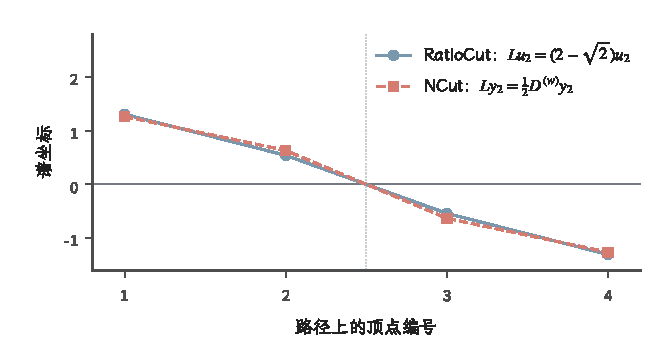
\includegraphics[width=\linewidth]{figures/01-mathematical-preliminaries/03-graphs-and-signals/matplotlib/teaching-graph/spectral-coordinates.pdf}
  \caption{单位权四顶点路径的两种谱方向。蓝实线为组合拉普拉斯第二特征向量，
  红虚线为度加权广义特征向量，点形也作区分。显示时均按欧氏范数\(2\)缩放，
  不替代NCut的度加权范数。横轴为四个离散顶点，连线仅引导阅读；
  竖虚线标出零阈值分割，两种方向虽同号分组，相对幅度并不相同。}
  \label{fig:graph-theory-spectral-coordinates}
\end{figure}

取整以后必须回到原离散目标核验质量。特征向量的方向稳定性还依赖相邻特征值间隔：
与其他特征值的间隔很小时，小扰动可能使方向明显旋转；
重特征值时应考察对应子空间，只有它与其余谱充分分离时才能谈相应稳定性，
不能把任意单个基向量当成固有划分。

\subsection{离散选择的近似与质量验证}

前面的谱划分已经展示了通用做法：扩大可行域获得下界，
再恢复原约束下的方案获得上界。仅把\(z_i\in\{0,1\}\)改成\(z_i\in[0,1]\)
还没有完整指定松弛，必须说明连续域上的目标怎样定义。
记原可行集为\(\mathcal Z\)，选
\(\widetilde{\mathcal Z}\supseteq\mathcal Z\)及延拓\(\widetilde{\mathcal E}\)，要求
\[
  \widetilde{\mathcal E}(\bm z)=\mathcal E(\bm z)\quad(\bm z\in\mathcal Z).
\]
则
\[
  L_{\mathrm{relax}}
  =\inf_{\bm z\in\widetilde{\mathcal Z}}\widetilde{\mathcal E}(\bm z)
  \leq \mathcal E^\star
  =\min_{\bm z\in\mathcal Z}\mathcal E(\bm z).
\]
不同延拓即使在离散点上一致，也可能得到不同下界。
若松弛最优值达到，且存在一个松弛最优解属于原可行集，它同时就是离散全局最优解；
分数解则还需要取整、局部搜索或分支定界。

恢复出可行配置\(\widehat{\bm z}\)以后，令\(U=\mathcal E(\widehat{\bm z})\)，
任何有效下界\(L\leq\mathcal E^\star\)都给出
\[
  0\leq U-\mathcal E^\star\leq U-L.
\]
\(U-L\)是次优差距的上界，不是实际误差；仅在下界紧时二者相等。
数值求解器当前的连续可行目标通常是松弛最优值的上界，
不能未经对偶证书或误差控制就把它称为原问题下界。
逐坐标按\(1/2\)阈值取整也可能破坏总数、连通等全局约束；
必须先检查恢复方案可行，才有上界\(U\)。

确定性取整需要逐实例的质量证明。采用随机取整时，还须利用后续
第~\ref{chap:random-variables}章的概率工具说明抽样规则、平均误差与修复可行性的代价；
本节的上下界证书则逐个检查所得到的方案。非负且\(\mathcal E^\star>0\)时，
\(U\leq\alpha\mathcal E^\star\)表达乘法近似比；目标可能为负或最优值为零时，
加法误差\(U-\mathcal E^\star\leq\varepsilon\)更适合。
运行快、连续目标下降与离散方案已最优是不同结论。

\section{图上的函数与传播}
\label{sec:graph-theory-functions-propagation}

图上“每点一个数”与“每种配置一个数”有不同定义域。
前者是\(f:V\to\mathbb R\)，四顶点图只需四个值；
后者是\(F:\mathcal Z_1\times\cdots\times\mathcal Z_4\to\mathcal S\)，
四个二值变量已有\(16\)种配置。
对前者汇总邻居，会改变一个顶点信号；对后者汇总变量，会产生边缘表或最优值。
二者都能沿图局部计算，却不能据此互换含义。

\subsection{顶点函数的变换与传播}
\label{sec:graph-theory-vertex-functions}
\label{sec:graph-theory-structure-comparison}

顶点数值可以表达温度、得分或某个观测通道；顶点标记则可以表达类别或局部结构类型。
数值允许线性叠加，离散标记未必有加法，因此分别使用谱变换和邻域细化。
重编号只是坐标改变，两种运算都需要检查是否随顶点同步重排。

\subsubsection{数值信号的谱变换与局部传播}
\label{sec:signal-analysis-graph-state-kernels}

一个\term{图信号}（graph signal）是给每个顶点一个数的函数，
固定编号后写成\(\bm f\in\mathbb R^n\)。
规则序列可以统一向前平移一步，一般图却没有唯一的全局“下一个顶点”。
这里回用第~\ref{sec:graph-theory-vertex-configuration}节的组合拉普拉斯，
用沿边变化的能量确定适合本图的坐标，而不预设规则时间轴上的傅里叶公式。

谱定理给出
\[
  \bm L=\bm U\bm\Lambda\bm U^\top,\qquad
  \bm U^\top\bm U=\bm I,\qquad
  \bm\Lambda=\operatorname{diag}(\lambda_1,\ldots,\lambda_n).
\]
其中\(0=\lambda_1\leq\cdots\leq\lambda_n\)。
\begin{definition}[图傅里叶变换]
  \label{def:signal-analysis-graph-fourier-transform}
  选定\(\bm L\)的一组实标准正交特征向量作为\(\bm U\)的列，
  图信号的\term{图傅里叶变换}（graph Fourier transform）及逆变换为
  \begin{equation}
    \widehat{\bm f}_{\mathcal G}=\bm U^\top\bm f,\qquad
    \bm f=\bm U\widehat{\bm f}_{\mathcal G}.
    \label{eq:signal-analysis-graph-fourier}
  \end{equation}
\end{definition}

正交性使变换不丢信息，并有
\[
  \|\bm f\|_2^2=\sum_{k=1}^n|\widehat f_{\mathcal G,k}|^2,\qquad
  \bm f^\top\bm L\bm f
  =\sum_{k=1}^n\lambda_k|\widehat f_{\mathcal G,k}|^2.
\]
所以小特征值的单位模态沿边变化较小，大特征值的单位模态变化较大，
这就是把\(\lambda_k\)称为图频率尺度的根据。
若有重特征值，对应空间内可旋转正交基，单个坐标随之改变，
该子空间上的投影及系数平方和却不变。图频率先对应特征空间，
不总是一个唯一的特征向量；即使简单特征值的实特征向量也有正负号自由度。

单位权简单环提供与规则序列相接的例子。取\(N\geq3\)，
顶点局部编号\(r=0,\ldots,N-1\)，每点连到模\(N\)的左右邻居。
这里的模态指标\(k=0,\ldots,N-1\)按复指数编号，不按前面的特征值大小排序。
直接计算
\[
  (\bm L\bm f)[r]=2f[r]-f[(r-1)\bmod N]-f[(r+1)\bmod N].
\]
令\(u_k[r]=N^{-1/2}e^{2\pi\mathrm i kr/N}\)，则
\begin{align*}
  (\bm L\bm u_k)[r]
  &=\left(2-e^{-2\pi\mathrm i k/N}-e^{2\pi\mathrm i k/N}\right)u_k[r]\\
  &=\left(2-2\cos\frac{2\pi k}{N}\right)u_k[r].
\end{align*}
不同\(k\)的内积为有限几何和：
\(\frac1N\sum_{r=0}^{N-1}e^{2\pi\mathrm i(k-\ell)r/N}\)
在\(k=\ell\)时为\(1\)，否则为\(0\)。
故这些模式组成复酉基，坐标变换用\(\bm U^*\bm f\)，逆变换用\(\bm U\)，
不能把实情形的转置直接用于复基。这些复指数模式与前章
定义~\ref{def:signal-analysis-dft}中的DFT使用同一组振荡函数；这里以
\(N^{-1/2}\)归一化基向量，所以图谱系数等于相应DFT系数除以\(\sqrt N\)。
直接代入环图算子并检查正交性，说明同一组模式为何既适合循环平移，也适合环图能量。
\(N=2\)时简单图的左右邻居重合，不能继续把该单边图写成度为\(2\)的上述环算子。

环图的\(k\)和\(N-k\)具有相同特征值，因而图能量并不区分两种复振荡方向。
一般图的模式还依赖连接、边权和归一化选择；
两个不同图上的第\(k\)个系数没有天然相同的物理频率。
跨图比较须依赖共同图构造、谱区间或子空间语义，不能仅按坐标序号对齐。

谱坐标建立以后，可以按标量响应\(g\)放大或缩小不同模态：
\[
  g(\bm L)=\bm U g(\bm\Lambda)\bm U^\top,\qquad
  \bm y=g(\bm L)\bm f,\qquad
  \widehat y_{\mathcal G,k}=g(\lambda_k)\widehat f_{\mathcal G,k}.
\]
相同特征值必须使用相同标量响应，所以\(g(\bm L)\)不依赖重特征空间内的任意基选择。
若对同一特征值的不同基向量随意赋不同系数，得到的就不是这个标量矩阵函数。

若响应是\(K\)次多项式，
\begin{equation}
  g(\bm L)=\sum_{r=0}^K\alpha_r\bm L^r,
  \label{eq:graph-theory-polynomial-filter}
\end{equation}
则滤波写成
\begin{equation}
  \bm y=\sum_{r=0}^K\alpha_r\bm L^r\bm f.
  \label{eq:signal-analysis-polynomial-graph-filter}
\end{equation}
一次乘\(\bm L\)只使用本点和一跳邻居的值。
归纳地，若\((\bm L^r)_{i,j}\neq0\)，矩阵乘积中必须存在至多\(r\)步的支撑图行走
从\(i\)到\(j\)，对角因子允许停留；因此图距离大于\(K\)时滤波矩阵条目为零。
“至多\(K\)跳”是依赖范围上界，不保证范围内每点的系数非零，
因为权重和多项式系数可能相消。
给定稀疏图及多项式系数，反复乘矩阵即可计算，无需显式对角化；
每步成本为\(O(|V|+|E_+|)\)。

三顶点路径的例子同时检验数值和范围：
\[
  \bm L=
  \begin{bmatrix}1&-1&0\\-1&2&-1\\0&-1&1\end{bmatrix},\qquad
  \bm f=(1,0,0)^\top,\qquad g(\lambda)=1-\lambda/3.
\]
于是
\[
  \bm H\bm f=(\bm I-\bm L/3)\bm f=(2/3,1/3,0)^\top.
\]
首点的数值只到一跳邻居。该图特征值为\(0,1,3\)，响应为\(1,2/3,0\)，
所以同一操作在谱坐标中消除了最高频模式。
再作用一次，
\[
  \bm H^2\bm f
  =(\bm I-2\bm L/3+\bm L^2/9)\bm f=(5/9,1/3,1/9)^\top,
\]
第三点才收到非零值，符合二次多项式的两跳范围。

\begin{figure}[htbp]
  \centering
  \begingroup
\begin{tikzpicture}[x=1mm,y=1mm,text=FigureInk,
  font=\figurefont\footnotesize,
  vertex/.style={circle,draw=FigureStroke,fill=white,line width=.9pt,
    minimum size=7mm,inner sep=0pt},
  existing/.style={vertex,fill=FigureBlueFill},
  reached/.style={vertex,fill=FigureRedFill},
  edge/.style={draw=FigureStroke,line width=1pt},
  note/.style={inner sep=0pt,fill=none}
]
  \path[use as bounding box] (0,0) rectangle (112,72);
  \foreach \y/\operator in {60/{\bm f},37/{\bm H\bm f},14/{\bm H^2\bm f}} {
    \node[note,anchor=east] at (24,\y) {\(\operator\)};
  }
  \node[existing] (a0) at (42,60) {\(1\)};
  \node[vertex] (b0) at (68,60) {\(2\)};
  \node[vertex] (c0) at (94,60) {\(3\)};
  \node[existing] (a1) at (42,37) {\(1\)};
  \node[reached] (b1) at (68,37) {\(2\)};
  \node[vertex] (c1) at (94,37) {\(3\)};
  \node[existing] (a2) at (42,14) {\(1\)};
  \node[existing] (b2) at (68,14) {\(2\)};
  \node[reached] (c2) at (94,14) {\(3\)};
  \foreach \r in {0,1,2} {
    \draw[edge] (a\r) -- (b\r) -- (c\r);
  }
  \foreach \x/\y/\value in {
    42/52/1,68/52/0,94/52/0,
    42/29/{2/3},68/29/{1/3},94/29/0,
    42/6/{5/9},68/6/{1/3},94/6/{1/9}} {
    \node[note] at (\x,\y) {\(\value\)};
  }
\end{tikzpicture}
\endgroup

  \caption{三顶点路径上的一次与二次局部滤波。顶点下方为精确值，
  白色表示零值，浅蓝表示此前已非零的顶点，浅红表示本步新到达的顶点；
  初始非零点也用浅蓝标出。颜色不编码连续色标。
  图的边均为单位权无向边，没有时间箭头；从上行到下行表示反复作用
  \(\bm H=\bm I-\bm L/3\)。两步结果的算子是二次多项式，能到达两跳邻居。}
  \label{fig:graph-theory-polynomial-locality}
\end{figure}
\FloatBarrier

这种谱滤波有时也称图卷积，但一般没有规则网格上那种唯一的核平移。
改变图或改用归一化拉普拉斯，同一个\(g\)会产生不同空间作用。
局部多项式只是本图算子的函数，不自动继承普通平移卷积的全部性质。

还要检查编号是否影响结果。顶点级输出应随重编号同步重排，称为等变；
整图级输出应保持相同，称为不变，完整定义见
定义~\ref{def:geometry-equivariant-map}和定义~\ref{def:geometry-invariant-map}。
对第~\ref{sec:graph-theory-graph-isomorphism}节的置换矩阵\(\bm P\)，
\begin{equation}
  \begin{aligned}
    \bm W'&=\bm P\bm W\bm P^\top,\qquad
    \bm D^{(w)\prime}=\bm P\bm D^{(w)}\bm P^\top,\\
    \bm L'&=\bm P\bm L\bm P^\top.
  \end{aligned}
  \label{eq:graph-theory-laplacian-relabel}
\end{equation}
若\(\bm f'=\bm P\bm f\)，则\(\bm L'\bm f'=\bm P\bm L\bm f\)。
更一般地，由\(\bm P^\top\bm P=\bm I\)相邻消去，
\[
  g(\bm L')\bm f'
  =\sum_{r=0}^K\alpha_r(\bm P\bm L\bm P^\top)^r\bm P\bm f
  =\bm P g(\bm L)\bm f.
\]
故多项式滤波等变；后接对顶点求和等对称读出，就得到不变的图级表示。
不变性只排除任意编号的影响，不保证不同非同构图一定得到不同结果。

有限次滤波每次最多增加有限跳数；连续时间扩散则把局部差分累计成矩阵指数。
若每点按邻居与自身的差调整，
\(f_i'(t)=\sum_jw_{i,j}(f_j(t)-f_i(t))\)，就得到
\begin{equation}
  \frac{\mathrm d\bm f(t)}{\mathrm dt}=-\bm L\bm f(t),\qquad
  \bm f(0)=\bm f_0.
  \label{eq:graph-theory-heat-equation}
\end{equation}
第~\ref{chap:matrix-analysis}章的矩阵指数给出
\[
  \bm f(t)=e^{-t\bm L}\bm f_0
  =\sum_{k=1}^ne^{-t\lambda_k}
    \langle\bm u_k,\bm f_0\rangle\bm u_k.
\]
各坐标独立按\(e^{-t\lambda_k}\)衰减，零模保持，大特征值模式衰减更快。
对任一支撑连通分量\(C\)，常量单位向量为\(\bm1_C/\sqrt{|C|}\)，
其投影在每点的值为\(|C|^{-1}\sum_{i\in C}f_{0,i}\)。
其余正特征值项趋于零，所以每个分量分别趋于自己的初始平均；
支撑连通时才是全图同一平均。

守恒和耗散也可不经对角化验证。由\(\bm1^\top\bm L=\bm0^\top\)，
\[
  \frac{\mathrm d}{\mathrm dt}\bm1^\top\bm f(t)
  =-\bm1^\top\bm L\bm f(t)=0.
\]
平方范数与Dirichlet能量不能混称为同一个能量：
\[
  \frac{\mathrm d}{\mathrm dt}\frac12\|\bm f(t)\|_2^2
  =\bm f(t)^\top\bm f'(t)
  =-\bm f(t)^\top\bm L\bm f(t)\leq0.
\]
边差能量的导数则为
\begin{align*}
  \frac{\mathrm d}{\mathrm dt}\bigl[\bm f(t)^\top\bm L\bm f(t)\bigr]
  &=\bm f'(t)^\top\bm L\bm f(t)+\bm f(t)^\top\bm L\bm f'(t)\\
  &=-2\bm f(t)^\top\bm L^2\bm f(t)
   =-2\|\bm L\bm f(t)\|_2^2\leq0.
\end{align*}
对称性保证两项相同。平方范数下降率等于负边差能量，
边差能量本身的下降率又多一个拉普拉斯，两个结论各有不同内容。

贯穿图取单位边权、\(\bm f_0=(1,0,0,0)^\top\)，其谱为\(0,2,4,4\)。
不同模态的保留比例为\(1,e^{-2t},e^{-4t}\)，重特征值\(4\)的两个方向同速衰减。
图连通且总和为\(1\)，所以极限为每点\(1/4\)，不是全部数值归零。

\begin{figure*}[htbp]
  \centering
  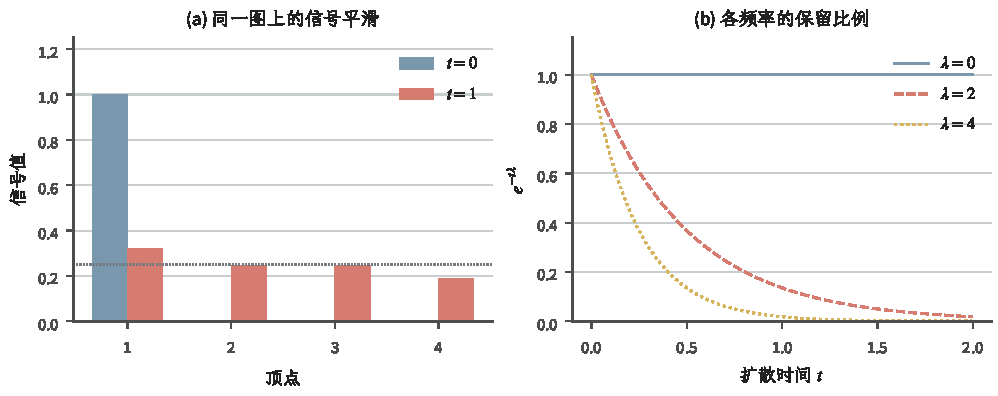
\includegraphics[width=\linewidth]{figures/01-mathematical-preliminaries/03-graphs-and-signals/matplotlib/probability-discrete/graph-diffusion-spectrum.pdf}
  \caption{贯穿四顶点图的解析式扩散。左图比较\(\bm f(0)=(1,0,0,0)^\top\)
  与\(\bm f(1)=e^{-\bm L}\bm f(0)\)，灰虚线是最终均值\(1/4\)；
  右图绘制特征值\(0,2,4\)的保留比例，\(4\)的重数为\(2\)。
  柱和曲线直接由该图的拉普拉斯计算，不表示实验均值或误差条。}
  \label{fig:graph-diffusion-spectrum}
\end{figure*}

指数一般不是固定低阶多项式，因此不能把有限次滤波的固定跳数截断套到它上面。
扩散使总边差能量不增，却不保证每条边两端的差都单调缩小。
例如单位权路径\(1-2-3\)从\(\bm f(0)=(1,1,0)^\top\)出发时，
\(\bm f'(0)=-\bm L\bm f(0)=(0,-1,1)^\top\)。
边\(1-2\)的初始差为零，差的导数却为\(1\)，因此短时间内两端会从相等变为不等；
此时总边差能量的导数仍为\(-4\)。整体耗散与逐边单调是两个不同的要求。
扩散也不保证保留预测所需的类别边界，时间过长会抹去同一支撑分量内的全部非恒定差异。

图Dirichlet能量还与第~\ref{chap:differential-geometry-and-symmetry}章的连续能量
\[
  \int_{\mathcal M}\|\operatorname{grad}f\|_g^2\,\mathrm dV_g
\]
形成离散与连续的对应：前者比较采样点之间的有限差分，
后者累计无穷小方向的变化。但形式相似不构成收敛定理。
若图来自点云，采样密度、邻域半径或核带宽、权重缩放、归一化及边界条件
共同决定可能的极限。邻域太大可能连接流形不同折，太小则可能断连；
未校正的不均匀采样可能导出带密度漂移的算子，
而不是仅由Riemann体积确定的Laplace--Beltrami算子。
离散谱结论相对于已选图精确成立，连续近似和任务语义仍各需额外条件。

\subsubsection{离散标记的邻域细化}

数值滤波考察信号变化，结构比较则常需知道各点周围有哪些类型的邻居。
只记录出现过哪些类型会丢掉次数；按编号排列又依赖任意顺序。
\term{多重集合}（multiset）保留种类与次数、忽略排列：
\(\{\!\{a,a,b\}\!\}\)与\(\{\!\{a,b\}\!\}\)不同。

\begin{definition}[一维邻域标记细化]
  \label{def:graph-theory-wl-refinement}
  一维Weisfeiler--Leman细化（1-dimensional Weisfeiler--Leman refinement, 1-WL）
  从初始标记\(c_i^{(0)}\)出发，同步更新
  \begin{equation}
    c_i^{(t+1)}=\operatorname{HASH}\left(
      c_i^{(t)},\left\{\!\left\{c_j^{(t)}:j\in N(i)\right\}\!\right\}
    \right),
    \label{eq:graph-theory-wl-refinement}
  \end{equation}
  其中\(\operatorname{HASH}\)对不同输入对给出不同新标记。
\end{definition}

这里是无碰撞编码的数学约定，不是普通有限哈希函数永不碰撞的承诺。
比较两图时必须共享初始标记规则和编码对应，
例如在两图的不交并上统一编码，不能各自随意命名后比较字面值。
同构只重排顶点及其邻居，所以每轮标记同步重排，各标记出现次数不变。
上述版本仅用无向邻域；有向或带边属性的细化需要相应扩充输入，不能无声丢掉方向和属性。

令\(\mathcal P^{(t)}\)为相同标记构成的分区。
更新包含自身旧标记，所以旧标记不同的两点下一轮仍不同；
\(\mathcal P^{(t+1)}\)只能细分，不能合并。
每次严格细分至少增加一个非空块，而\(n\)点最多有\(n\)块，
因此严格细分至多\(n-1\)次。
若某轮分区未变，同一块中的顶点已有相同的各旧块邻居计数，
给这些块统一换新标记不会改变计数相等性，下一轮也不能再拆分，
归纳可知以后一直稳定。稳定指等价类不再细分，符号名称仍可换新。

稳定不等于已判定同构。所有顶点初始同标记时，六环\(C_6\)与两个不相连三角形
都让每点看到两个同标记邻居，归纳地每轮仍同标记，两图各有六个此类顶点。
1-WL无法区分它们，尽管前者连通、后者不连通。

\begin{figure}[htbp]
  \centering
  \begingroup
% Local styles; callers keep this input inside a group.
\tikzset{
  reader vertex/.style={circle,draw=FigureStroke,fill=white,line width=1pt,
    minimum size=7mm,inner sep=0pt,font=\figurefont\footnotesize,text=FigureInk},
  reader factor/.style={rectangle,draw=FigureStroke,fill=FigureYellowFill,
    line width=1pt,minimum size=8mm,inner sep=2pt,font=\figurefont\footnotesize},
  reader edge/.style={draw=FigureStroke,line width=1.1pt},
  reader arrow/.style={reader edge,-{Stealth[length=2.2mm,width=1.4mm]}},
  reader label/.style={font=\figurefont\footnotesize,text=FigureInk},
  reader note/.style={reader label,fill=white,inner sep=1pt},
  reader highlight/.style={draw=FigureYellow,line width=1.1pt},
  reader auxiliary/.style={draw=FigureMuted,line width=0.6pt,dashed}
}

\begin{tikzpicture}[text=FigureInk]
  \node[reader label] at (0,1.7) {(a) 六顶点环 \(C_6\)};
  \foreach \i in {1,...,6}
    \node[reader vertex,fill=FigureYellowFill] (a\i) at ({90-60*(\i-1)}:1.1) {};
  \foreach \i/\j in {1/2,2/3,3/4,4/5,5/6,6/1}
    \draw[reader edge] (a\i)--(a\j);
  \node[reader label] at (5.2,1.7) {(b) 两个不相交三角形};
  \foreach \x/\prefix in {3.8/b,6.6/c}
  {
    \node[reader vertex,fill=FigureYellowFill] (\prefix1) at (\x,0.9) {};
    \node[reader vertex,fill=FigureYellowFill] (\prefix2) at (\x-0.75,-0.6) {};
    \node[reader vertex,fill=FigureYellowFill] (\prefix3) at (\x+0.75,-0.6) {};
    \draw[reader edge] (\prefix1)--(\prefix2)--(\prefix3)--(\prefix1);
  }
  \node[reader label] at (0,-1.85) {每个顶点：2个同标记邻居};
  \node[reader label] at (5.2,-1.85) {每个顶点：2个同标记邻居};
\end{tikzpicture}
\endgroup

  \caption{同样的邻居标记计数可以来自不同全局结构。两张六顶点图初始同标记，
  每轮每点仍见到两个同标记邻居，故1-WL计数无法区分一条六环与两个三角形。
  这不表示连通性难计算，而是说明该细化遗漏了这一差异。
  浅黄只表示共同标记，不加入唯一编号，以保持无标记图的比较设定。}
  \label{fig:graph-theory-wl-local-ambiguity}
\end{figure}

给每个顶点附任意唯一编号不是无条件补救：若重编号后重新按编号赋特征，
输出会依赖命名；若把额外属性随置换同步移动，可以保持等变，
但问题已变成带属性图的比较。
具体图网络的共享更新、聚合和读出能否达到或超过某种细化的区分能力，
还须在模型章节依据函数族证明。结构等变性不等于完全可辨，更不等于泛化保证。

\subsection{配置函数的汇总与查询}
\label{sec:graph-theory-semiring-dynamic-programming}

现在每个顶点\(i\)代表变量\(z_i\)，取值于非空有限集合\(\mathcal Z_i\)；
贯穿例取\(\mathcal Z_i=\{0,1\}\)。
配置函数\(F(\bm z)\)评价全部变量的一次完整赋值。
图记录哪些变量同时进入局部函数，查询则另行规定要输出总权重、最优值，
还是保留部分变量的函数表。只有明确输出以后，“消去变量”才有确定含义。

\subsubsection{配置查询的目标与半环运算}

先不谈分解，直接看两变量表
\[
  g(x,y)=
  \begin{array}{c|cc}
    &y=0&y=1\\ \hline
    x=0&1&3\\
    x=1&2&4
  \end{array}.
\]
若数字是非负权重，总权重与最佳权重分别为
\[
  \sum_{x,y}g(x,y)=10,\qquad \max_{x,y}g(x,y)=4.
\]
最佳权重的见证为\((1,1)\)。
若同一数字解释为成本，最低成本为\(1\)，见证变为\((0,0)\)。
关系图相同，甚至表也相同，仍不能替读者决定查询。

若输出要保留\(y\)，求和消去\(x\)得到
\(m(y)=\sum_xg(x,y)\)，即\(m(0)=3,m(1)=7\)。
这是一张表，再汇总\(y\)才得标量\(10\)。
将每格权重除以\(10\)，得到给各对\((x,y)\)分配份额的联合概率表；
各格非负，全部份额相加为\(1\)。把具有同一\(y\)的份额相加，得到只记录\(y\)
的边缘概率，所以这里\(y=0,1\)的概率分别是\(3/10,7/10\)。
这一步只需对有限表求和；一般概率分布将在第~\ref{chap:random-variables}章定义。
若改为最大化，得到\(m(0)=2,m(1)=4\)，记录每个\(y\)的最佳权重，
不再是边缘概率。消元是汇总内部变量的贡献，不是删除它的约束。

为某个固定配置组合局部项，与跨不同配置汇总结果，是两种操作。
普通权重用乘法组合、加法汇总；成本用加法组合、最小值汇总。
分别记为\(\otimes\)和\(\oplus\)，核心规则是：不依赖被汇总变量的项可移到汇总外。

\begin{definition}[交换半环]
  \label{def:graph-theory-semiring}
  本章使用的交换\term{半环}（semiring）记为
  \[
    (\mathcal S,\oplus,\otimes,e_{\oplus},e_{\otimes}),
  \]
  包含一个集合、两种运算及其单位元。
  两种运算分别结合且交换，单位元分别为\(e_{\oplus}\)、\(e_{\otimes}\)，并满足
  \[
    a\otimes(b\oplus c)=(a\otimes b)\oplus(a\otimes c),\qquad
    a\otimes e_{\oplus}=e_{\oplus}.
  \]
  空汇总取\(e_{\oplus}\)，空组合取\(e_{\otimes}\)。
\end{definition}

半环不要求加法逆元或乘法逆元；这里的局部算法不需减法和除法。
几个具体实例为
\[
  \begin{array}{c|c|c|c|c}
    \text{用途}&\mathcal S&\oplus&\otimes&(e_{\oplus},e_{\otimes})\\ \hline
    \text{总权重}&\mathbb R_{\geq0}&+&\times&(0,1)\\
    \text{最大权重}&\mathbb R_{\geq0}&\max&\times&(0,1)\\
    \text{最小成本}&\mathbb R\cup\{+\infty\}&\min&+&(+\infty,0)\\
    \text{是否可行}&\{\mathrm{false},\mathrm{true}\}&\lor&\land&
       (\mathrm{false},\mathrm{true})
  \end{array}
\]
最大积中的\(0\)既是最大值运算的单位元，也是乘法吸收元。
最小加法约定\(+\infty+c=+\infty\)，用正无穷表达不可行。
对数域还可用\((\mathbb R\cup\{-\infty\},\max,+,-\infty,0)\)，
约定\(-\infty+c=-\infty\)。这些选择改变答案，不能只当成实现细节。

再引入局部因子。贯穿图上的一元与成对专门情形为
\begin{equation}
  F(\bm z)=\bigotimes_{i\in V}\phi_i(z_i)
    \otimes\bigotimes_{\{i,j\}\in E}\phi_{i,j}(z_i,z_j).
  \label{eq:graph-theory-factorized-objective}
\end{equation}
因子是局部函数，作用域是它依赖的变量集合。
若要表达原三元子句，仍须保留\(\phi_{2,3,4}(z_2,z_3,z_4)\)；
上述成对公式不是从三个两两关系恢复三元约束的等价式。
一般可写\(F(\bm z)=\bigotimes_a\phi_a(\bm z_{S_a})\)，
其中\(S_a\subseteq V\)为任意有限作用域。
改变作用域会改变分解和计算成本，即使某些数值条目恰好相同。

例如和积下要保留\(z_4\)，查询为
\[
  Q(z_4)=\sum_{z_1,z_2,z_3}F(\bm z),\qquad
  Z=\sum_{z_4}Q(z_4).
\]
只有在\(F\)是非负权重且\(0<Z<\infty\)时，\(F/Z\)才为每个完整配置分配
非负且总和为\(1\)的概率，\(Q(z_4)/Z\)才是只保留\(z_4\)的边缘概率。
若总权重为零，就不能作这种归一化。若改问最低成本，目标为
\(\min_{\bm z}[\sum_i c_i(z_i)+\sum_{\{i,j\}\in E}c_{i,j}(z_i,z_j)]\)，
就须同时更换组合和汇总。图本身不自动添加概率、因果或时间语义。

\subsubsection{基于变量消元的查询与恢复}

第~\ref{sec:graph-theory-elimination-width}节已说明消元如何改变作用域，
现在证明它如何保持数值查询。
每次收集全部含\(z_i\)的当前因子\(\mathcal F_i\)，合并其作用域并去掉\(i\)，
记剩余接口为\(R_i\)，生成
\[
  \psi_i(\bm z_{R_i})
  =\bigoplus_{z_i\in\mathcal Z_i}\ \bigotimes_{f\in\mathcal F_i}f.
\]
删去这些旧因子，以\(\psi_i\)替换；其余因子保持不动。
这不是丢掉\(z_i\)的影响，而是对每个剩余接口值预先算出它的全部贡献。
完整消元的目标，在贯穿成对例中为
\begin{equation}
  Z=\bigoplus_{\bm z\in\mathcal Z_1\times\cdots\times\mathcal Z_4}
  \left[
    \bigotimes_i\phi_i(z_i)
    \otimes\bigotimes_{\{i,j\}\in E}\phi_{i,j}(z_i,z_j)
  \right].
  \label{eq:graph-theory-semiring-elimination}
\end{equation}

\begin{theorem}[半环变量消除的正确性]
  \label{thm:graph-theory-semiring-elimination}
  对有限取值变量和交换半环，按任意完整次序对有限个局部因子执行上述消元，
  所得标量等于直接枚举的全局汇总。
  特别地，式~\eqref{eq:graph-theory-factorized-objective}得到
  式~\eqref{eq:graph-theory-semiring-elimination}。
  若保留一组输出变量，在其余变量消去后停止，所得表逐个输出配置等于原查询。
\end{theorem}

\begin{proof}
维持更强的不变量：对每个尚未消去变量的固定配置，
当前因子的半环组合等于原函数对已消去变量的汇总。
初始没有已消变量，不变量即为原局部分解。

设下一变量是\(z_i\)，把当前因子分成含它的\(\mathcal F_i\)和不含它的
\(\mathcal F_{-i}\)。固定其他变量，有限性和分配律给出
\[
  \bigoplus_{z_i}
  \left[
    \left(\bigotimes_{f\in\mathcal F_{-i}}f\right)
    \otimes\left(\bigotimes_{f\in\mathcal F_i}f\right)
  \right]
  =
  \left(\bigotimes_{f\in\mathcal F_{-i}}f\right)
  \otimes\left(\bigoplus_{z_i}\bigotimes_{f\in\mathcal F_i}f\right).
\]
右侧最后一项就是新因子\(\psi_i\)。结合律与交换律允许把对\(z_i\)的汇总
接在此前已消变量的有限汇总之后，因而新的当前组合等于原函数对全部已消变量的汇总，
不变量保持。
若再对剩余变量汇总，上式也表明每一步的全局值不变：
\begin{align*}
  &\bigoplus_{\bm z_{-i}}\bigoplus_{z_i}
    \left[\left(\bigotimes_{f\in\mathcal F_{-i}}f\right)
       \otimes\left(\bigotimes_{f\in\mathcal F_i}f\right)\right]\\
  &\qquad=\bigoplus_{\bm z_{-i}}
    \left[\left(\bigotimes_{f\in\mathcal F_{-i}}f\right)\otimes\psi_i\right].
\end{align*}
归纳到所有变量消去，只剩直接枚举的标量。
若输出变量不消去，同一逐配置不变量即给出所需函数表。
\end{proof}

正确性允许任意次序，中间表成本却不相同。
贯穿图先消去\(1,4\)只需保留接口\(\{2,3\}\)；
先消去\(2\)则形成对\(\{1,3,4\}\)的表，并出现填充边\(\{1,4\}\)。
结构部分给出的\(q^{k+1}\)工作表界因此控制实际消元，而不改变查询定义。

和积得到的是未归一化权重；保留输出变量后仍需除以同一总权重，
并检查总权重严格为正。最大积则得到
\[
  M=\max_{\bm z}\prod_i\phi_i(z_i)
        \prod_{\{i,j\}\in E}\phi_{i,j}(z_i,z_j).
\]
只存最大值不能恢复最优配置。
每次对接口配置保存一个达到最大值的\(z_i\)，最后从末次选择开始，
按消元逆序用已知接口值查回选择，即能恢复一个全局见证。
每一步都保存条件最优选择，反向代入使该步达到原先记录的局部最优值，
归纳便得到全局值\(M\)。并列时须声明固定平局规则、返回任意一个或枚举全部；
枚举全部的输出规模可能很大。

最小加法同理求得
\[
  C^\star=\min_{\bm z}
    \left[\sum_i c_i(z_i)+\sum_{\{i,j\}\in E}c_{i,j}(z_i,z_j)\right],
\]
并保存条件最小选择回溯；若最优值为\(+\infty\)，就应报告没有有限成本可行配置。
严格正权重可用负对数把最大积转成最小加法，
因为乘积变为和，负对数反转大小次序。
零权重约定映为\(+\infty\)，负权重则没有直接的实对数解释；
若用普通对数，得到的是最大加法而非最小加法。

同一种有限汇总可换序，不同汇总通常不行。
取
\[
  h(x,y)=
  \begin{array}{c|cc}
    &y=0&y=1\\ \hline
    x=0&4&0\\
    x=1&0&4
  \end{array}.
\]
要求先固定同一个\(x\)、再累计全部\(y\)，得到
\begin{equation}
  \max_x\sum_yh(x,y)=4.
  \label{eq:graph-theory-max-sum-order-a}
\end{equation}
允许每个\(y\)分别选择最佳\(x\)，则为
\begin{equation}
  \sum_y\max_xh(x,y)=8.
  \label{eq:graph-theory-max-sum-order-b}
\end{equation}
区别是是否允许选择随\(y\)而改变。
一般对有限实值表，
\[
  \max_x\sum_yh(x,y)\leq\sum_y\max_xh(x,y),
\]
因为对任意固定\(x\)，每个\(h(x,y)\leq\max_{x'}h(x',y)\)，
相加再最大化仍保序。
若某个共同\(x\)在所有\(y\)上同时最大，显然取等号；
反过来，若取等号，取左侧一个最优\(x\)，逐项非负差的总和为零，
故每项都为零，也就必须有这样一个共同最优选择。

混合求和与最大化因此限制合法消元次序，最小可用宽度可能超过普通树宽。
按配置份额求和得到边缘概率、直接寻找权重最大的完整配置，以及先求和再对保留变量
最大化，是不同的查询，不能混用目标或消元次序。
把有限和改成连续积分，还须回用定理~\ref{thm:analysis-tonelli-fubini}：
在\(\sigma\)有限乘积测度下，非负可测函数可由Tonelli换序，
带符号函数通常需要Fubini的绝对可积条件。
把求和号改成积分号不自动保证存在性、换序或有限表算法仍适用。

\subsubsection{基于树形消息的局部查询}

消元把内部变量压缩成接口表；树消息则按固定的树形接口复用这些表。
在贯穿图的一元与成对情形中，先消去\(z_1\)所得表为
\begin{equation}
  m_{1\to\{2,3\}}(z_2,z_3)=
  \bigoplus_{z_1\in\mathcal Z_1}
  \phi_1(z_1)\otimes\phi_{1,2}(z_1,z_2)\otimes\phi_{1,3}(z_1,z_3).
  \label{eq:graph-theory-interface-message}
\end{equation}
同样计算\(z_4\)一侧的\(m_{4\to\{2,3\}}\)，
再在接口上组合两条消息与\(\phi_2,\phi_3,\phi_{2,3}\)，最后汇总\(z_2,z_3\)。
若还有三元因子\(\phi_{2,3,4}\)，应把它完整纳入\(4\)侧表。
每种接口配置的局部结果只算一次。

合法性的直接原因是分配律，而不只是图形看起来分成两侧。
对不依赖\(z_1\)的项\(c(z_2,z_3)\)，
\[
  \bigoplus_{z_1}\bigl(c(z_2,z_3)\otimes g(z_1,z_2,z_3)\bigr)
  =c(z_2,z_3)\otimes\bigoplus_{z_1}g(z_1,z_2,z_3).
\]
图确定哪些项与内部变量无关，半环公理允许移出汇总，
接口表则保存可复用的子问题答案。

先在一棵树上严格定义消息。顶点放一元因子，边放成对因子；
删去\(\{u,v\}\)，记\(u\)侧连通分量为\(T_{u\mid v}\)。
消息不是只汇总顶点\(u\)，而是汇总整棵\(u\)侧子树：
\begin{equation}
  \begin{aligned}
    m_{u\to v}(z_v)
    =\bigoplus_{\bm z_{T_{u\mid v}}}
    \biggl[
      &\bigotimes_{i\in T_{u\mid v}}\phi_i(z_i)\\[-2pt]
      {}\otimes&
      \bigotimes_{\substack{\{i,j\}\in E\\i,j\in T_{u\mid v}}}
        \phi_{i,j}(z_i,z_j)
      \otimes\phi_{u,v}(z_u,z_v)
    \biggr].
  \end{aligned}
  \label{eq:graph-theory-tree-message-semantics}
\end{equation}
唯一保留的自变量为接口值\(z_v\)，跨接口边项也必须计入。

\begin{theorem}[树消息递推]
  \label{thm:graph-theory-tree-message-recursion}
  对有限取值变量、有限树及交换半环，上述消息满足
  \begin{equation}
    m_{u\to v}(z_v)=\bigoplus_{z_u}
    \left[
      \phi_u(z_u)\otimes\phi_{u,v}(z_u,z_v)
      \otimes\bigotimes_{r\in N(u)\setminus\{v\}}m_{r\to u}(z_u)
    \right].
    \label{eq:graph-theory-tree-message-recursion}
  \end{equation}
\end{theorem}

\begin{proof}
对子树\(T_{u\mid v}\)大小归纳。若\(u\)为叶顶点，没有入消息，空组合为单位元，
递推就是对\(\phi_u\otimes\phi_{u,v}\)汇总\(z_u\)，与定义相同。
若还有邻居\(r\neq v\)，删除\(u\)后，各\(T_{r\mid u}\)互不重叠，
彼此无边；否则会破坏树的唯一路径性质。
归纳假设将每个这样的子树连同通往\(u\)的边概括为\(m_{r\to u}(z_u)\)。
结合律与交换律允许按子树分组，分配律把仅依赖\(z_u,z_v\)的项移到
各子树汇总之外，再汇总\(z_u\)，便得到递推式。
每个顶点因子、内部边因子和接口边因子都被计入恰好一次。
\end{proof}

任取根\(r\)，从叶到根汇集消息以后，
\[
  Z=\bigoplus_{z_r}\left[\phi_r(z_r)\otimes
      \bigotimes_{u\in N(r)}m_{u\to r}(z_r)\right].
\]
不汇总\(z_r\)就得到根的查询表；再把消息从根发回各枝，
可在每个顶点组合全部入消息，得到相应未归一化边缘表或条件最优表。
和积的归一化与最优查询的选择回溯仍遵循上一小节，消息本身不替代这些步骤。

一般图可先用树分解或团树形成袋。
每个因子作用域在原始图中成团，团入袋性质保证能把因子完整分配给一个包含它的袋，
并且只分配一次。记袋\(B\)的因子组合为\(\Phi_B\)，
相邻袋\(B,C\)的接口为\(S_{B,C}=B\cap C\)，递推为
\[
  m_{B\to C}(\bm z_{S_{B,C}})
  =\bigoplus_{\bm z_{B\setminus S_{B,C}}}
    \left[
      \Phi_B(\bm z_B)\otimes
      \bigotimes_{D\in N_{\mathcal T}(B)\setminus\{C\}}
        m_{D\to B}(\bm z_{D\cap B})
    \right].
\]
运行交集保证：若某变量同时出现在删去树边后的两侧，
它必属于该边接口；若出现在两个相邻子树，也必经过当前袋。
因此固定袋配置就为每个入消息指定一致接口值，袋外内部变量彼此分离，
可以沿用子树归纳。运行交集失效时，同一变量可能在两枝被独立取不同值，
这正是无效树分解会破坏查询的原因。

贯穿图中叶袋\(\{1,2,3\}\)向袋\(\{2,3,4\}\)发送关于\(z_2,z_3\)的表，
后者组合自己的一元或高阶因子完成查询。
若分解宽度为\(k\)、每变量至多\(q\)个状态，枚举袋配置至多用\(q^{k+1}\)项，
接口表通常更小；还须计入原始因子读取、袋数和每次半环运算成本。
给定袋数为多项式量级的正确分解、固定\(k,q\)、可有效计算的局部表及运算，
整体才有关于顶点数的多项式保证。寻找最优树分解本身是另一问题，
宽度随顶点数增长时也没有这个固定参数保证。

在原始有环图上直接反复发送树形公式的消息，某个局部项可能经不同路线返回，
造成重复计数；子树互不重叠的证明已经失效。
这种循环消息可作为近似方法研究，但是否收敛、收敛到什么及误差多大都须另证。
有限次邻域传播、图信号扩散和配置查询至此都有明确语义，
不能仅因它们都沿边通信就互相替代。

\section{本章小结}
\label{sec:graph-theory-summary}

回到开篇的四顶点图，\(1\)与\(4\)虽不相邻，却可以经\(2\)或\(3\)到达。
图保留了这种关系结构，却没有替三元子句保存真值表，也没有决定边是长度、容量还是相似度。
无向可达性可以用遍历回答；有向条件分离则须检查全部底层路径的活跃性。
祖先道德化为单次查询转换图，只有满足弦图与完美性条件时，
才存在保留全部分离答案的固定等价表示。概率独立仍需要相应模型假设。

接口\(\{2,3\}\)使左右两侧能够分开计算，但“能够分块”还不够。
生成树只保留连接骨架，可能改变距离、环和分离关系；
消元保留后续作用域，却可能产生填充。
贯穿图先处理\(1,4\)的宽度为\(2\)，先处理\(2\)则增至\(3\)。
树分解的运行交集保证接口配置相容，树宽控制能达到的最小袋规模；
状态数、因子访问成本和允许的消元次序共同决定实际计算量。

加入目标以后，还须逐项检查最优性的条件。
非负边长支持Dijkstra永久确定距离，DAG则依赖无环次序而允许负边；
最大流与同值割给出上下界相遇的证书，MST依赖割交换，
二部匹配利用整数流，二值次模能量利用非负割表示。
表~\ref{tab:graph-algorithm-conditions}将这些条件与可核对的输出放在一起。

\begin{table*}[htbp]
  \centering
  \caption{图查询的目标、关键条件与正确性依据。有限输入编码和数值误差仍须在实现中检查；
  同一张图可提出多种查询，一种目标的最优解不自动解决其他目标。}
  \label{tab:graph-algorithm-conditions}
  \begin{tabular}{p{0.20\linewidth}p{0.33\linewidth}p{0.37\linewidth}}
    \toprule
    问题与算法 & 关键条件 & 输出与正确性依据\\
    \midrule
    Dijkstra最短路 & 所有边长非负 & 单源距离与前驱；最小暂定距离的归纳不变量\\
    Bellman--Ford & 允许负边；区分可达负环的后继 & 有限距离、不可达或\(-\infty\)；
      有限边数递推与影响范围\\
    最小生成树 & 无向连通图；成本可正可负 & 最小总成本连接树；割交换性质\\
    最大流与最小割 & 非负有限容量、流守恒 & 可行流与同值割共同认证最优\\
    二部最大匹配 & 二部图、端点互斥、基数目标 & 整数单位容量流；无增广路径的割证书\\
    树分解动态规划 & 运行交集、有限状态、合法半环与次序 &
      精确配置查询；时间指数依赖袋大小，还需计入状态数和运算成本\\
    二值能量最小割 & 有限一元/成对成本；每个成对项次模 &
      能量与非负割容量仅差常数，返回全局最优配置\\
    \bottomrule
  \end{tabular}
\end{table*}

缺少精确结构时，先给出原问题可行解，再与有效松弛下界比较。
RatioCut按顶点数平衡，NCut按度体积平衡，因而松弛后的特征方程不同。
连续坐标须取整并回到离散目标核验；上界与下界之差只给出次优差距的上界。

图函数的定义域决定传播在做什么。
顶点数值借助图傅里叶坐标按模态变换，多项式滤波限制有限跳数，
热扩散则最终保留每个正权支撑分量的平均，可能抹去任务所需差异。
顶点标记的1-WL细化虽然等变，却不能区分六环与两个三角形；
编号无关不等于结构完全可辨。配置函数则依赖半环分配律，
由消元与树消息精确汇总内部变量，不能用普通邻域数值聚合替代。

前章第~\ref{chap:signal-analysis}章利用规则时间或位置索引建立傅里叶表示与卷积，
本章再用图连接与沿边能量选择模态和传播规则。环图把两种坐标联系起来，
一般图却没有统一平移或天然一致的物理频率，不能直接照搬规则信号的全部性质。
后续第~\ref{chap:random-variables}章将为权重和观测建立概率描述，
第~\ref{chap:causal-inference}章再区分图的分离判据与概率、生成机制中的独立关系。
